\graphicspath{{2limits/asy/}}

\section{Sequences}
\setcounter{subsection}{6}

Sequences are the fundamental tool in our approach to analysis.

\subsection{Limits of Sequences}

\begin{defn}{}{sequence}
	A \emph{sequence} of real numbers is a list indexed by the natural numbers
	\[
		(s_n)=(s_1,s_2,s_3,\ldots)
	\]
	We call $s_1$ the \emph{initial term/element.}
\end{defn}

More formally, we could view a sequence as a function $s_n:\N\to\R$. Other letters may be used ($a_n,b_n$, etc.), though $s_n$ is typical in the abstract. It is also common to have sequences which start with a different initial term (e.g., $n=0$). If you need to be explicit, write, e.g., $(s_n)_{n=0}^\infty$.


\begin{examples}{}{easylimits}
	\exstart Explicit sequences are often defined by providing a formula for the $n\th$ term. For instance, $s_n=\left(1+\frac 1n\right)^n$ defines a sequence whose first three terms are
	\[
		s_1=2,\quad s_2=\tfrac 94,\quad s_3=\tfrac{64}{27},\quad\ldots
	\]
	Since each term is a rational number, $(s_n)$ could be described as a \emph{rational sequence.}
	\begin{enumerate}\setcounter{enumi}{1}
	  \item\label{ex:easylimits2} Sequences can be defined inductively. For instance, if $t_1=1$ and $t_{n+1}=3t_n-1$, then
	  \[
	  	(t_n)=(1,2,5,14,41,\ldots)
	  \]
	  \item $u_n=\frac 1{n^2-4}$ defines a sequence with initial term $u_3=\frac 15$:
	  \[
	  	(u_n)_{n=3}^\infty =\bigl(\tfrac 15,\tfrac 1{12},\tfrac 1{21},\ldots\bigr)
	  \]
	\end{enumerate}
\end{examples}


\boldinline{Limits}

We are typically most interested in what happens to the terms of a sequence when $n$ gets \emph{large} (one reason it is common to be non-explicit as to the initial term). In elementary calculus you should have become used to examples such as\footnote{%
	If there are multiple letters around, writing $\lim\limits_{n\to\infty}$ with a subscript can aid the reader.%
}
\[
	\lim\frac{2n^2+3n-1}{3n^2-2}=\frac 23
\]
which encapsulates the idea that the expression $s_n=\frac{2n^2+3n-1}{3n^2-2}$ gets close to $\frac 23$ when $n$ is large. We can easily convince ourselves of this with a calculator/computer: to 4 decimal places,
\[
	(s_n)=\bigl(4,\,1.3,\,1.04,\,
 	0.9348,\,
 	0.8767,\,
 	0.8396,\,
 	0.8138,\,
 	0.7947,\,\ldots\bigr),\qquad 
 	s_{1000}=0.6677
\]
Our primary business is to make this idea logically watertight. In the next section we will do so by developing the formal definition of limit. Before seeing this, we quickly refresh a few simple examples. All these example can be made formal later, but for the present just rely on your intuition and experience: it is essential to have a good idea of the correct answer \emph{before} you try to prove it!

\goodbreak

\begin{examples}{}{}
	\exstart $\lim \frac 1n=0$. Our instinct is that $s_n=\frac 1n$ becomes arbitrarily small as $n$ becomes large. 
	\begin{enumerate}\setcounter{enumi}{1}
	  \item $\lim\frac{7n+9}{2n-4}=\frac 72$. To convince yourself of this, you might write $\frac{7n+9}{2n-4}=\frac{7+\frac 9n}{2-\frac 4n}$
	  and observe that the $\frac 1n$ terms become tiny as $n$ increases.
	  \item The sequence with $n\th$ term $s_n=(-1)^n$ does not converge to anything: it \emph{diverges}.
	  \[
	  	(s_n)_{n=0}^\infty=(1,-1,1,-1,1,-1,\ldots)
	  \]
	  \item If $c_n=\frac 1n\cos\left(\frac{\pi n}6\right)$, then $\lim c_n=0$. To see this, observe that the cosine term lies between $\pm 1$, while $\frac 1n$ has limit 0.
	  \item The sequence defined inductively by $s_0=2$, \ $s_{n+1}:=\frac 12s_n+3$ begins
	  \[
	  	(s_n)=\bigl(2,4,5,\tfrac{11}2,\tfrac{23}4,\tfrac{47}8,\ldots\bigr)
	  \]
	  This appears to have limit $\lim s_n=6$. It is not hard to spot the pattern $s_n=6-\frac{4}{2^n}$, which may easily be verified by induction: for the induction step, observe that
	  \[
	  	\frac 12s_n+3=\frac 12\left(6-\frac 4{2^n}\right) +3 =6-\frac 4{2^{n+1}}
	  \]
	\end{enumerate}
\end{examples} 


%	\lim_{n\to\infty}\sqrt{n^2+4}-n=\lim_{n\to\infty}\frac 4{\sqrt{n^2+4}+n}=0

%\vfil

\begin{exercises}{}{}
	\emph{Key concepts/results:\quad Sequence,\quad Use your intuition!}
	
	\begin{enumerate}
	  \item%[2.]
	  Decide whether each sequence converges; if it does, state the limit. No proofs are required; if you're unsure what's going on, try writing out the first few terms.
		\begin{enumerate}
	    \item \makebox[100pt][l]{$a_n=\dfrac 1{3n+1}$\hfill (b) }\ 
	    \makebox[100pt][l]{$b_n=\dfrac{3n+1}{4n-1}$\hfill (c) }\ 
	    \makebox[100pt][l]{$c_n=\dfrac n{3^n}$\hfill (d) }\ 
	    $d_n=\sin\left(\dfrac{n\pi}4\right)$
	  \end{enumerate}

	  
	  \item Repeat the previous question for sequences whose $n\th$ term is as follows:
	  \begin{enumerate}
	    \item \makebox[85pt][l]{$\dfrac{n^2+3}{n^2-3}$\hfill (b) }\ 
	    \makebox[85pt][l]{$1+\dfrac 2n$\hfill (c) }\ 
	    \makebox[85pt][l]{$2^{1/n}$\hfill (d) }\ 
	    \makebox[85pt][l]{$(-1)^nn$\hfill (e) }\
			$\dfrac{7n^3+8n}{2n^3-31}$
	    \setcounter{enumii}{5}
	    \item \makebox[85pt][l]{$\sin\left(\dfrac{n\pi}2\right)$\hfill (g) }\ 
	    \makebox[85pt][l]{$\sin\left(\dfrac{2n\pi}3\right)$\hfill (h) }\ 
	    \makebox[85pt][l]{$\dfrac{2^{n+1}+5}{2^n-7}$\hfill (i) }\ 
	    \makebox[85pt][l]{$\left(1+\dfrac 1n\right)^2$\hfill (j) }\ 
	    $\dfrac{6n+4}{9n^2+7}$
	  \end{enumerate}

	  
	  \item Give an example of:
	  \begin{enumerate}
		  \item A sequence $(x_n)$ of irrational numbers having a limit $\lim x_n$ that is a rational number.
		  \item A sequence $(r_n)$ of rational numbers having a limit $\lim r_n$ that is an irrational number.
	  \end{enumerate}
	  
	  
	  \item Prove by induction that the sequence defined in Example \ref*{ex:easylimits}.\ref{ex:easylimits2} has $n\th$ term $t_n=\frac 12\bigl(3^{n-1}+1\bigr)$.
	  
	  
	  \item In future courses, you'll meet sequences of \emph{functions.} For instance,  we could define a sequence $(f_n)$ of functions $f_n:\R\to\R$ inductively via
	  \[
	  	f_0(x)\equiv 1,\qquad f_{n+1}(x):=1+\int_0^x f_n(t)\,\dt
	  \]
	  Compute the functions $f_1,f_2$ and $f_3$. The sequence $(f_n)$ should seem familiar if you think back to elementary calculus; why?
	\end{enumerate}
\end{exercises}


\clearpage

\iffalse


\subsection{The Formal Definition of Limit}\label{sec:limitdef}


\begin{defn}{}{limit}
A sequence $(s_n)$ \emph{converges to a limit $s\in\R$}, if\footnotemark
\[\forall\epsilon>0,\ \exists N\ \text{such that}\ n>N\implies \nm{s_n-s}<\epsilon\]
We write $\lim s_n=s$ or simply $s_n\to s$; both are read ``$s_n$ \emph{approaches} (or \emph{tends to}) $s$."\smallbreak
A sequence \emph{converges} if it has a limit, and \emph{diverges} otherwise.
\end{defn}

\footnotetext{$N$ can be quantified as either a real or a natural number, the definitions being equivalent by the Archimedean property: if $N\in\R$ satisfies the definition, then $\exists\widetilde N\in\N$ such that $\widetilde N\ge N$; but then $n>\widetilde N\implies n>N\ldots$ It tends to be easier to use $\R$ for convergence and $\N$ when directly proving \emph{divergence} (see Definition \ref{defn:divergence1}).}

This isn't as hard as it looks! The best way to understand it is to work a \emph{lot} of examples\ldots

 %Observe how $\epsilon$ measures how \emph{close} the sequential values $s_n$ are to the limit $s$; no matter how small we make $\epsilon$, there is some \emph{tail} of the sequence (all $s_n$ with $n>N$) whose terms are less than $\epsilon$ from the limit.


% Below is a clickable version\footnote{If you want to the picture to move, you'll need to open these notes in a full-function pdf reader such as Acrobat. A lightweight pdf viewer or a web-broswer will likely only show a single still frame.} of the limit definition for the sequence with $n^\text{th}$ term
% \[s_n=1+\frac 32e^{-n/20}\cos\frac n4\]
% You should believe without proof that $s=\lim s_n=1$. Try viewing the definition as a game:
% \begin{quote}
% Given \textcolor{blue}{$\epsilon>0$}, we \emph{choose} $N$ so that all terms \textcolor{orange}{$s_n$} coming \emph{after} $N$ are closer to $s$ than $\epsilon$.
% \end{quote}

% \begin{center}
% \animategraphics[controls]{4}{_limitdefanim}{0}{16}
% \end{center}

\goodbreak


\begin{example}{}{}
We show that the sequence with $n\th$ term $s_n=2-\frac 1{\sqrt n}$ converges to $s=2$.\smallbreak

If we plot the sequence like a function, we see how $\epsilon$ controls the distance from $s_n$ is to the limit $s$; the definition requires us to show that no matter how small we make $\epsilon$, there is some \textcolor{orange}{tail} of the sequence (all $s_n$ with $n>N$) whose terms are less than a distance $\epsilon$ from the limit.\vspace{-5pt}

\begin{center}
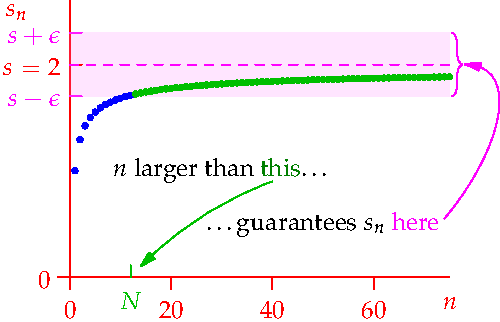
\includegraphics[scale=0.9]{limitdef-pic}\vspace{-8pt}
\end{center}

To verify a `for all, there exists' statement requires an argument with a specific structure:
\begin{itemize}\itemsep0pt
  \item Suppose $\epsilon>0$ has been provided and describe $N$, dependent on $\epsilon$ (\href{http://www.math.uci.edu/~ndonalds/math140a/limitdefanim.html}{$\epsilon$ smaller means $N$ larger}).
  \item Verify algebraically that $n>N\implies\nm{s_n-s}<\epsilon$.
\end{itemize}

\emph{Scratch work.}\quad To find a suitable $N$, start with what you want to be true and let it inspire you.
\begin{quote}
We want $\nm{s_n-s}=\nm{\left(2-\frac 1{\sqrt n}\right)-2} =\nm{\frac 1{\sqrt n}}<\epsilon$ (equivalently $n>\frac 1{\epsilon^2}$) whenever $n>N$. Choosing $N=\frac 1{\epsilon^2}$ should be enough to complete the proof!
\end{quote}
\textcolor{red}{Warning!}\quad We do not yet have a proof: ``$N=\frac 1{\epsilon^2}$'' is not the correct conclusion! We finish by rearranging our scratch work to make it clear that the definition is satisfied.\medbreak

\emph{Formal argument.}\quad
Suppose $\epsilon>0$ is given, and let $N=\frac 1{\epsilon^2}$. Then
\[
n>N\implies \nm{s_n-s}=\nm{2-\frac 1{\sqrt n}-2} =\frac 1{\sqrt n}<\frac 1{\sqrt N}=\epsilon
\]
Thus $s_n\to 2$, as required.
\end{example}

%\footnotetext{A linked  illustrates this.}

\goodbreak




The last three lines are all we need---think of them as the concert performance after much rehearsal! With practice, you might be able to do simple $\epsilon$--$N$ arguments like these without scratch work, though even experts usually require some.\smallbreak

Before seeing more examples, we prove a hopefully intuitive result.

\begin{lemm}{Uniqueness of Limit}{}
If $(s_n)$ converges, then its limit is unique.
\end{lemm}

The proof structure should be familiar from other uniqueness arguments: assume there are two limits $s\neq t$ and obtain a contradiction. The picture explains the strategy: by choosing $\epsilon=\frac{\nm{s-t}}2$ in the definition we obtain a \emph{tail} of the sequence (all terms $s_n$ coming \emph{after} some $N$) which must be simultaneously close to \emph{both limits.}
\begin{center}
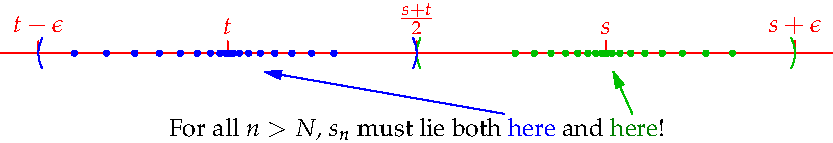
\includegraphics{limitunique}
\end{center}

\begin{proof}
Suppose $s\neq t$ are two limits. Take $\epsilon=\frac{\nm{s-t}}2$ and apply Definition \ref{defn:limit} twice: $\exists N_1,N_2$ such that
\[n>N_1\implies \nm{s_n-s}<\frac{\nm{s-t}}2\quad \text{and}\quad n>N_2\implies \nm{s_n-t}<\frac{\nm{s-t}}2\]
Define $N:=\max\{N_1,N_2\}$. Then,
\begin{align*}
n>N\implies\nm{s-t}=\nm{s-s_n+s_n-t}&\le\nm{s_n-s}+\nm{s_n-t} \tag*{($\triangle$-inequality)}\\
&<\frac{\nm{s-t}}2+\frac{\nm{s-t}}2 =\nm{s-t}
\end{align*}
Contradiction.
\end{proof}


\begin{examples}{}{moreeasylimits}
	We give several more examples of using the limit definition. Remember that only the formal arguments needs to be presented; some scratch work is included to show the thought process.
	
	\begin{enumerate}
		\item\label{ex:stdzero} For any $k\in\R^+$, we prove that $\lim\frac 1{n^k}=0$.
		\smallbreak
		
		\emph{Scratch work.}\quad Given $\epsilon>0$, we want to choose $N$ such that
		\[n>N\implies \frac 1{n^k}<\epsilon\]
		This amounts to having $n>\frac 1{\epsilon^{1/k}}$, so it is enough to choose $N$ to be the right hand side.
		\smallbreak
		
		\emph{Formal argument.}\quad Let $\epsilon>0$ be given, and let $N=\frac 1{\epsilon^{1/k}}$. Then
		\[
		n>N \implies \nm{\frac 1{n^k}-0}=\frac 1{n^k}<\frac 1{N^k}=\epsilon
		\]
		We conclude that $\frac 1{n^k}\to 0$, as required.
	
		\goodbreak
		
		
		\item We prove that $\lim \bigl(\sqrt{n+4}-\sqrt n\bigr) =0$.
		\smallbreak
		
		\emph{Scratch work.}\quad Everything follows from a (hopefully) familiar algebraic trick for manipulating surd expressions:
		\[\sqrt{n+4}-\sqrt n=\frac 4{\sqrt{n+4}+\sqrt n} <\frac 4{2\sqrt n}=\frac 2{\sqrt n}\]
		
		\emph{Formal argument.}\quad Let $\epsilon>0$ be given, and let $N=\frac 4{\epsilon^2}$. Then
		\[n>N\implies \nm{\sqrt{n+4}-\sqrt n}=\frac 4{\sqrt{n+4}+\sqrt n} <\frac 4{2\sqrt n}=\frac 2{\sqrt n}<\frac 2{\sqrt N}=\epsilon\]
		Thus $\lim\bigl(\sqrt{n+4}-\sqrt n\bigr) =0$, as required.

	\item\label{ex:ep2} We prove that $\lim\frac{3n+1}{n-7}=3$.
		\smallbreak
	
		\emph{Scratch work.}\quad Given $\epsilon>0$, we want to choose $N$ such that
		\[n>N\implies \nm{\frac{3n+1}{n-7}-3}=\nm{\frac{(3n+1)-3(n-7)}{n-7}}=\nm{\frac{22}{n-7}}<\epsilon \tag{$\ast$}\]
		For large $n$ ($n>7$) everything is positive, so it is sufficient for us to have
		\[n-7>\frac{22}\epsilon\quad\text{or equivalently}\quad n>7+\frac{22}{\epsilon}\]
		\smallbreak
		
		\emph{Formal argument 1.}\quad Let $\epsilon>0$ be given, and let $N=7+\frac{22}{\epsilon}$. Then
		\[n>N\implies \nm{\frac{3n+1}{n-7}-3} =\frac{22}{n-7} <\frac{22}{N-7}=\epsilon\]
		The absolute values are dropped since $n>7$. We conclude that $\lim\frac{3n+1}{n-7}=3$.
		\medbreak
		
		\emph{Scratch work (cont).}\quad An alternative approach is available if we play with ($\ast$) a little. By insisting that $n\ge 14$, we may simplify the denominator
		\[n-7\ge \frac 12n\implies \frac{22}{n-7}\le \frac{22}{\frac 12n}=\frac{44}n\]
		\smallbreak
		
		\emph{Formal argument 2.}\quad Let $\epsilon>0$ be given, and let $N=\max\bigl\{14,\frac{44}{\epsilon}\bigr\}$. Then
		\begin{align*}
		n>N\implies \nm{\frac{3n+1}{n-7}-3}&=\nm{\frac{22}{n-7}}\le\frac{22}{\frac 12n} =\frac{44}n \tag{since $n\ge 14$}\\
		&<\frac{44}N \le\epsilon\tag*{(since $N\ge \frac{44}\epsilon$)}
		\end{align*}
		We again conclude that $\lim\frac{3n+1}{n-7}=3$.
		\bigbreak

		The plot illustrates the two choices of $N$ as functions of $\epsilon$. Observe how the second is always larger than the first: if $N=N_1(\epsilon)$ works in a proof, then any larger choice $N_2(\epsilon)$ will also,
		\[n>N_2\ge N_1\implies n>N\implies \nm{s_n-s}<\epsilon\]
		Use this to your advantage to produce simpler arguments.

		\begin{center}
			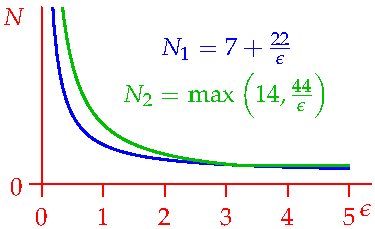
\includegraphics{epsilonNex}
		\end{center}

		\goodbreak
		
		
		

		\item\label{ex:conv3} Given $s_n=\frac{2n^4-3n+1}{3n^4+n^2+4}$, we prove that $\lim s_n=\frac 23$.\smallbreak
		
		\emph{Scratch work.}\quad We want to conclude that
		\[n>N\implies \nm{\frac{2n^4-3n+1}{3n^4+n^2+4}-\frac 23}=\nm{\frac{-2n^2-9n-5}{3(3n^4+n^2+4)}}<\epsilon\]
		Attempting to solve for $n$ (as in the first method previously) is crazy! Instead we simplify the fraction by observing that since $n\ge 1$, we have
		\begin{align*}
			\nm{\frac{-2n^2-9n-5}{3(3n^4+n^2+4)}} &\le\frac{16n^2}{3(3n^4+n^2+4)} \tag{$1\le n\le n^2$ and the $\triangle$-inequality}\\
			&<\frac{16n^2}{9n^4}<\frac 2{n^2} \tag{$n^2+4>0\implies 3n^4+n^2+4>3n^4$}
		\end{align*}
		The final simplification is merely for additional tidying.


		\emph{Formal argument.}\quad Let $\epsilon>0$ be given, and let $N=\sqrt{\frac 2\epsilon}$. Then
		\begin{align*}
			n>N\implies \nm{s_n-\frac 23}&=\nm{\frac{-2n^2-9n-5}{3(3n^4+n^2+4)}} <\frac{16n^2}{9n^4} \tag{since $n\ge 1$}\\
			&< \frac 2{n^2}<\frac 2{N^2}=\epsilon
		\end{align*}

		Other choices of $N$ are feasible (see e.g.{} Exercise \ref{exs:conv23again}); everything depends on how you want to simplify things in your scratch work.
		
	\end{enumerate}
\end{examples}

\vfil

\goodbreak

\boldsubsubsection{Divergent sequences}

By negating Definition \ref{defn:limit}, we obtain a new definition.

\begin{defn}{}{divergence1}
A sequence $(s_n)$ \emph{does not converge to $s\in\R$} if,
\[\exists \epsilon>0\ \text{such that}\ \forall N,\ \exists n>N\ \text{with}\ \nm{s_n-s}\ge\epsilon\]
A sequence is \emph{divergent} if it does not converge to \emph{any} limit $s\in\R$. Otherwise said,
\[\forall s\in\R,\ \exists \epsilon>0\ \text{such that}\ \forall N,\ \exists n>N\ \text{with}\ \nm{s_n-s}\ge\epsilon\]
\end{defn}

% We made one tiny change when negating Definition \ref{defn:limit}: $N$ is now a \textcolor{red}{natural number}.\footnote{Thanks to the Archimedean principle, replacing $N\in\R$ with $N\in\N$ results in an \emph{equivalent definition} of limit: if $N\in\R$ satisfies the definition, then $\exists\tilde N\in\N$ such that $\tilde N\ge N$. Certainly $n>\tilde N\implies n>N$\ldots} The advantage of this approach will become clear momentarily.



\begin{examples}{}{divergenceeasy}
	\exstart We prove that the sequence with $s_n=\frac 7n$ does not converge to $s=2$.
	\begin{enumerate}\setcounter{enumi}{1}
	  \item[]\emph{Visualization.}\quad We intuitively know that $s_n\to 0$. If $\epsilon$ is anything smaller than 2, then the terms $s_n$ will eventually be further than this from $s=2$.
	  \begin{center}
  		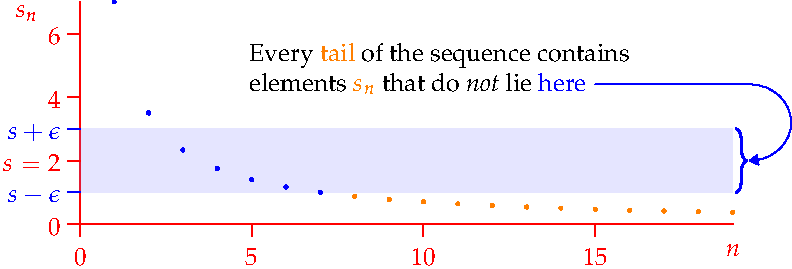
\includegraphics[scale=0.9]{divergent}
  	\end{center}
  	\vspace{-5pt}
	  
  	\emph{Direct argument.}\quad Let $\epsilon=1$. Since we are only concerned with \emph{large} values of $n$, we see that
  	\[\nm{s_n-s}=\nm{\frac 7n-2}=2-\frac 7n\ge \epsilon= 1\iff \frac 7n\le 1\iff n\ge 7\]
  	Given $N\in\N$, let\footnotemark{} $n=\max\{7,N+1\}$. But then $\nm{s_n-s}=\nm{\frac 7n-2}\ge\epsilon$, from which we conclude that $s_n\nrightarrow 2$.
  	\smallbreak
  	
  	\emph{Contradiction argument.}\quad For an alternative approach, we suppose $s_n\to 2$ and let $\epsilon=1$ in Definition \ref{defn:limit}. Then $\exists N$ such that
  	\[n>N\implies \nm{\frac 7n-2}<1 \implies 1<\frac 7n<3\implies \frac 73<n<7\]
  	Regardless of the value of $N$, this cannot hold \emph{for all} $n>N$: in particular $n:=\max\{7,N+1\}$. Contradiction.
  	\smallbreak
  	
  	The two arguments are very similar, though consider that a significant advantage of the contradiction approach is that you only have to remember \emph{one definition}!
	\end{enumerate}

% 	\exstart We prove that the sequence with $s_n=\frac 7n$ does not converge to $s=1$.
% 	\begin{enumerate}\setcounter{enumi}{1}
% 	  \item[]\emph{Visualization.}\quad We intuitively know that $s_n\to 0$. If $\epsilon$ is smaller than 1 (say $\frac 12$), then the terms $s_n$ will eventually be further than this from $s=1$.
% 	  \begin{center}
%   		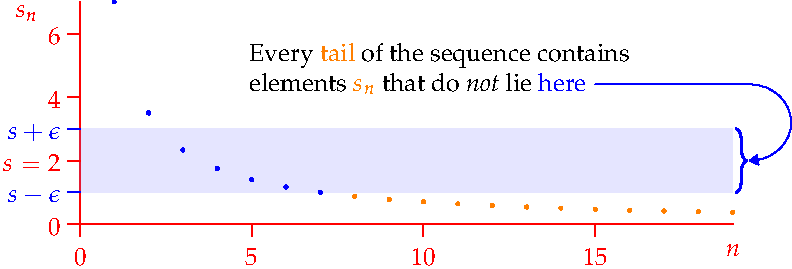
\includegraphics[scale=0.9]{divergent}
%   	\end{center}
%   	\vspace{-5pt}
% 	  
%   	\emph{Direct argument.}\quad Let $\epsilon=\frac 12$. Since we are only concerned with \emph{large} values of $n$, we see that
%   	\[\nm{s_n-s}=\nm{\frac 7n-1}=1-\frac 7n\ge\frac 12\iff 1-\frac 7n\ge\frac 12\iff \frac 7n\le\frac 12\iff n\ge 14\]
%   	Given $N\in\N$, let\footnotemark{} $n=\max\{14,N+1\}$. But then $\nm{s_n-s}=\nm{\frac 7n-1}\ge\epsilon$, from which we conclude that $s_n\nrightarrow 1$.
%   	\smallbreak
%   	
%   	\emph{Contradiction argument.}\quad For an alternative approach, we suppose $s_n\to 1$ and let $\epsilon=\frac 12$ in Definition \ref{defn:limit}. Then $\exists N$ such that
%   	\[n>N\implies \nm{\frac 7n-1}<\frac 12 \implies \frac 12<\frac 7n<\frac 32\implies \frac{14}3<n<14\]
%   	Regardless of the value of $N$, this cannot hold \emph{for all} $n>N$: in particular $n=\max\{14,N+1\}$. Contradiction.
%   	\smallbreak
%   	
%   	The two arguments are very similar, though consider that a significant advantage of the contradiction approach is that you only have to remember \emph{one definition}!
% 	\end{enumerate}
\end{examples}

\footnotetext{This is why we prefer to let $N$ be a natural number when proving divergence. If $N\in\R$, then we'd have to use the ceiling function ($n=\max\{14,\lceil N\rceil+1\}$), or resort to the Archimedean property on which it depends ($\exists n>\max\{14,N\}$). Either way is ugly and potentially confusing, so better avoided.} 

\goodbreak


\begin{tcolorbox}[exstyle]{}
	\begin{enumerate}\setcounter{enumi}{1}
		\item\label{ex:divergenceeasy2} We prove that the sequence defined by $s_n=(-1)^n$ is divergent.\smallbreak

		Suppose, for contradiction, that $s_n\to s$. The picture shows the case $s\ge 0$ and strongly suggests that $\epsilon=1$ will lead to a contradiction (why?).
		\begin{center}
   		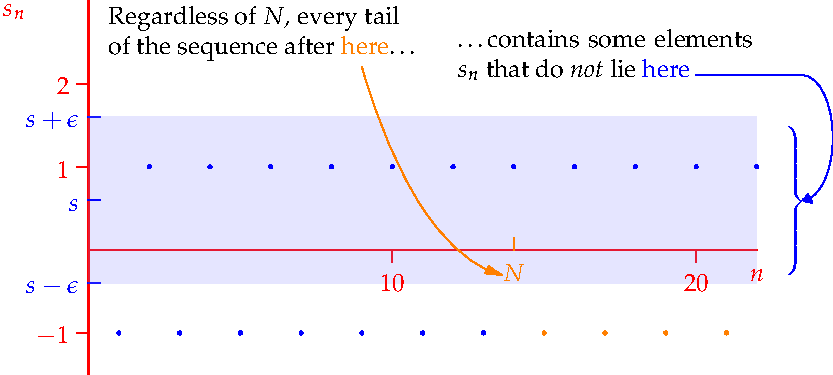
\includegraphics[scale=0.9]{divergent2}
  	\end{center}
   	Let $\epsilon=1$ in the definition of limit. Then $\exists N\in\N$ such that
		\[n>N\implies \nm{(-1)^n-s}<1\]
		One each of the values $\{\textcolor{magenta}{n_e},\textcolor{Green}{n_o}\}=\{N,N+1\}$ is \textcolor{magenta}{even} and the other \textcolor{Green}{odd}. There are two cases:
		\begin{itemize}
		  \item If $s\ge 0$ then $\nm{(-1)^{n_o}-s}=\nm{-1-s}=s+1\ge 1=\epsilon$.
		  \item If $s<0$ then $\nm{(-1)^{n_e}-s}=\nm{1-s}=1-s\ge 1=\epsilon$.
		\end{itemize}
		Either way we have a contradiction. We conclude that $(s_n)$ is divergent.

  
  	\item\label{ex:divergence3} We show that the sequence defined by $s_n=\ln n$ is divergent.\footnotemark\smallbreak
  		
		Our intuition from calculus is that logarithms increase unboundedly. For any $s\in\R$, letting $\epsilon=1$ should be enough, for eventually $\ln n\ge s+1$. This time we prove directly using the definition of divergence (\ref{defn:divergence1}).\smallbreak
		
		Suppose $s\in\R$, let $\epsilon=1$, and suppose that $N\in\N$ is given. Define $n=\max\{N+1,e^{s+1}\}$ and observe that. Then
		\[n>N\text{ and }\ln n\ge \ln(e^{s+1})=s+1 \tag{$\ln$ is \emph{increasing}, and so respects inequalities!}\]
		In particular,
		\[\nm{s_n-s}=\ln n-s\ge 1=\epsilon\]
		We conclude that $(s_n)$ is divergent.
	\end{enumerate}
\end{tcolorbox}

\footnotetext{In the next section we'll have a definition of what it means for a sequence to \emph{diverge to $\infty$}: this is what's happening for $s_n=\ln n$, but it's not (yet) what we're trying to demonstrate.}

\vfil
\goodbreak


\boldsubsubsection{A Little Abstraction}

Working explicitly with the limit definition is tedious. In the next section we'll develop and summarize the \emph{limit laws} so we can combine limits of sequences without providing new $\epsilon$-$N$ proofs. To start working towards this, here are three general results.

\begin{lemm}{}{ssquared}
If $\lim s_n=s$, then  $\lim s_n^2=s^2$.
\end{lemm}

The challenge is that we want to bound $\nm{s_n^2-s^2}=\nm{s_n-s}\nm{s_n+s}$, which means we need some control over $\nm{s_n+s}$. One way uses the triangle-inequality,
\[\nm{s_n+s}=\nm{s_n-s+2s}\le\nm{s_n-s}+2\nm s\]
Assuming $\nm{s_n-s}\le 1$ gives us a fixed bound $\nm{s+s_n}\le 1+2\nm s$. We may now begin a proof.

\begin{proof}
Suppose $s_n\to s$. Let $\epsilon>0$ be given, and let $\delta=\min\{1,\frac\epsilon{1+2\nm s}\}$. Since $s_n\to s$, $\exists N$ such that
\[n>N\implies \nm{s_n-s}<\delta\]
But then
\begin{align*}
n>N\implies \nm{s_n^2-s^2}&=\nm{s_n-s}\nm{s_n+s}\\
 %\overset{\triangle}{\le}
&\le\nm{s_n-s}\left(\nm{s_n-s}+2\nm s\right) \tag*{($\triangle$-inequality)}\\
&<\delta(1+2\nm s)\tag*{(since $\nm{s_n-s}<\delta\le 1$)}\\
&\le\epsilon\tag*{\qedhere}
\end{align*} 
\end{proof}


% \begin{proof}
% Observe that $\nm{s_n^2-s^2}=\nm{s_n-s}\nm{s_n+s}$. To bound this by $\epsilon$, we need to control the term $\nm{s_n+s}$. Return to the definition of limit with $\epsilon=1$: since $s_n\to s$ we know that $\exists M$ such that
% \begin{align*}
% n>M&\implies \nm{s_n-s}<1\implies -1+2s<s_n+s<1+2s\\
% &\implies \nm{s_n+s}<\max\{\nm{1+2s},\nm{-1+2s}\}
% \end{align*}
% Label the RHS of this last inequality $A$: we can now finish the argument.\\
% Let $\epsilon>0$ be given. Then $\exists P$ s.t. $n>P\implies \nm{s_n-s}<\frac\epsilon A$. Now let $N=\max\{M,P\}$. Then
% \[n>N\implies \nm{s_n^2-s^2}=\nm{s_n-s}\nm{s_n+s}<\frac\epsilon A\cdot A=\epsilon\tag*{\qedhere}\]
% \end{proof}

\begin{thm}{}{limitgreatk}
	Suppose $\lim s_n=s$.
	\begin{enumerate}
	  \item If $s_n\ge m$ for all except finitely many $n$, then $s\ge m$.
	  \item If $s_n\le M$ for all except finitely many $n$, then $s\le M$.
	\end{enumerate} 
\end{thm}

\begin{proof}
	We prove part 1 by contradiction---part 2 is similar.\smallbreak
	Suppose $s_n\to s<m$ and let $\epsilon=\frac{m-s}2>0$. Then $\exists N$ such that
	\begin{align*}
	n>N&\implies \nm{s_n-s}<\frac{m-s}2\implies s_n-s<\frac{m-s}2\\
	&\implies s_n-m<\frac{s-m}2<0\tag*{(add $s-m$ to both sides)}
	\end{align*}
	By assumption, $s_n<m$ holds for \emph{at most finitely many} $n$. Contradiction.
\end{proof}

The expression \emph{for all but finitely many $n$} can be added to many abstract limit theorems; other common variants are \emph{for all large $n$,} and \emph{for some tail of the sequence.} To avoid cumbersome language, the expression is often omitted. Remember that convergence/divergence is concerned with what happens when $n$ is \emph{large}: we can change or delete the first million terms of $(s_n)$ without altering it's convergence status!

\vfil\vfil
\goodbreak


\begin{thm}{Squeeze Theorem}{squeeze}
	Suppose three sequences satisfy $a_n\le s_n\le b_n$ (for all large $n$) and that $(a_n)$ and $(b_n)$ both converge to $s$. Then $\lim s_n=s$.
\end{thm}

\begin{proof}
	By subtracting $s$ from our assumed inequality, we see that
	\[a_n-s\le s_n-s\le b_n-s\implies\nm{s_n-s}\le\max\{\nm{a_n-s},\nm{b_n-s}\}\]
	It remains to bound the right hand side by $\epsilon$. Let $\epsilon>0$ be given, then there exist $N_a,N_b$ such that
	\[n>N_a\implies \nm{a_n-s}<\epsilon\quad\text{and}\quad n>N_b\implies \nm{b_n-s}<\epsilon\]
	Finally let $N=\max\{N_a,N_b\}$ to see that
	\[n>N\implies \nm{s_n-s}\le\max\{\nm{a_n-s},\nm{b_n-s}\}<\epsilon\tag*{\qedhere}\]
\end{proof}


\begin{example}{}{}
	If $s_n=\frac{1+\sin n}n$, then $0\le s_n\le \frac 2n$. The squeeze theorem quickly forces $\lim s_n=0$.
\end{example}

\vfil

\begin{exercises}{}{}
	\emph{Key concepts/results:\quad ????}

	\begin{enumerate}
	  \item For each sequence, determine the limit and prove your claim.
	  \begin{enumerate}
	    \item\makebox[120pt][l]{$a_n=\frac{n}{n^2+1}$\hfill (b)} \ \makebox[120pt][l]{$b_n=\frac{7n-19}{3n+7}$\hfill (c)} \ $c_n=\frac{4n+3}{7n-5}$
	    \setcounter{enumii}{3}
	    \item\makebox[120pt][l]{$d_n=\frac{2n+4}{5n+2}$\hfill (e)} \ \makebox[120pt][l]{$e_n=\frac 1n\sin n$\hfill (f)} \ $f_n=\frac{n^2+n-1}{3n^2-10}$
	  \end{enumerate}
	
	
	  \item\label{exs:tbddproduct}%[4.]
	  Let $(t_n)$ be a bounded sequence (there exists $M$ such that $\nm{t_n}\le M$ for all $n$), and let $(s_n)$ be a sequence such that $\lim s_n=0$. Prove that $\lim(s_nt_n)=0$.\par
	  (\emph{Hint: given $\epsilon$, note that $\frac\epsilon{\nm M}$ is also a small number\ldots})
	 
	 
	  \item%[8.]
	  Prove the following
	  \begin{enumerate}
		  \item $\lim[\sqrt{n^2+1}-n]=0$ \hspace{30pt} (b) \ $\lim[\sqrt{n^2+n}-n]=\frac 12$\hspace{30pt} (c) \ $\lim[\sqrt{4n^2+n}-2n]=\frac 14$
	  \end{enumerate}
	  
	
	  \item\label{exs:convlowerbound}%[10.]
	  Let $(s_n)$ be a convergent sequence, and suppose $\lim s_n>a$. Prove that there exists $N$ such that $n>N\implies s_n>a$.
	  
	    
	  \item\label{exs:conv23again}
	  \begin{enumerate}
	    \item Show that $n\ge 2\implies 2n^2+9n+5\le 9n^2$.
	    \item (Example \ref*{ex:moreeasylimits}.\ref{ex:conv3})\quad Give another proof that $\lim \frac{2n^4-3n+1}{3n^4+n^2+4}=\frac 23$ by choosing $N=\max\{2,\frac 1{\sqrt\epsilon}\}$.
	 	\end{enumerate}
	 	
	 	
	  \item\begin{enumerate}
	   	\item Prove that the sequence with $n\th$ term $s_n=\frac 2{n^2}$ does not converge to $-1$.
			\item Prove that $(s_n)$ does not converge to 1.
		\end{enumerate}
	    
	  \item Prove that the sequence defined by $t_n=n^2$ diverges.
	  
	 	
	 	\item Provide a contradiction argument to justify Example \ref*{ex:divergenceeasy}.\ref{ex:divergence3}: $(\ln n)$ diverges.
	
			
		\item (Recall Theorem \ref{thm:limitgreatk})\quad Suppose $\lim s_n=s$ where every $s_n>m$. Can we conclude that $s>m$? Explain your answer.
		
		
		\item\begin{enumerate}
			\item If $\nm{s_n-s}<1$, explain why $\nm{s_n^2+ss_n+s^2}< 1+3\nm s+3\nm s^2$
			\item Suppose $s_n\to s$. Prove that $s_n^3\to s^3$.  
		\end{enumerate}
		
	\end{enumerate}
\end{exercises}

\clearpage




\subsection{Limit Theorems for Sequences}

We'd like to develop some rules for working with limits so that we don't have to resort to an $\epsilon$--$N$ proof every time. The rough idea is that limits respect the basic rules of algebra. For instance\ldots

\begin{example}{}{}
If $\lim s_n=s$, it seems natural that a new sequence $(5s_n)$ obtained by multiplying the original terms by 5 should have limit $\lim 5s_n=5s$. Consider what we have to prove to confirm this:
\[\forall\epsilon>0, \exists N\text{ such that }n>N\implies \nm{5s_n-5s}<\epsilon\]
This last amounts to observing that $\nm{s_n-s}<\frac\epsilon 5$. The challenge here is to see that we're essentially done: this is just the statement $\lim s_n=s$ in disguise! Here is a more formal argument.\smallbreak
Let $\epsilon>0$ be given. Since $\lim s_n=s$, we know that
\[\exists N\text{ such that }n>N\implies \nm{s_n-s}<\frac\epsilon 5\implies \nm{5s_n-5s}<\epsilon\]
%We conclude that $\lim 5s_n=5s$.
\end{example}

The trick in the example will be used repeatedly in the proofs that follow. What's critical is that you read the limit definition correctly: given any small number ($\epsilon,\frac\epsilon 5$, etc.) there is some tail of the sequence which remains closer to the limit than this.

\begin{thm}{Limit laws}{limitbasic}
Limit calculations respect algebraic operations: $\pm, \times,\div$ and roots.\smallbreak
More specifically, if $(s_n)$ converges to $s$ and $(t_n)$ to $t$, then,
\begin{enumerate}
	%\item If $k\in\R$ is constant, then $\lim ks_n=ks$
	\item $\lim (s_n\pm t_n)=s\pm t$
	\item $\lim(s_nt_n)=st$; \ as a special case, if $k$ is constant, then $\lim ks_n=ks$
	\item If $t\neq 0$, then $\lim \frac{s_n}{t_n}=\frac st$
	\item If $k\in\N$, then $\lim \sqrt[k]{s_n}=\sqrt[k]{s}$, provided the roots exist ($s_n,s\ge 0$ if $k$ even)
\end{enumerate}
\end{thm}

Our first example was the special case of part 2 with $k=5$. Note also how parts 2 and 4 extend Lemma \ref{lemm:ssquared}: by induction we now have $s_n^q\to s^q$ for any $q\in\Q$.\smallbreak

Proving the limit laws takes a little work, including a small lemma. To advertise their benefit, we repeated apply them to a limit calculation as you might have seen it in elementary calculus.

\begin{examples}{}{methodmeanex}
\exstart We evaluate $\lim\frac{3n^2+2\sqrt n-1}{5n^2-2}$ using the limit laws.
\begin{align*}
\lim\frac{3n^2+2\sqrt n-1}{5n^2-2}&=\lim\frac{3+\frac 2{n^{3/2}}-\frac 1{n^2}}{5-\frac 2{n^2}} =\frac{\lim\left(3+\frac 2{n^{3/2}}-\frac 1{n^2}\right)}{\lim\left(5-\frac 2{n^2}\right)}\tag{part 3}\\
&=\frac{\lim 3+\lim\frac 2{n^{3/2}}-\lim\frac 1{n^2}}{\lim 5-\lim\frac 2{n^2}}\tag{part 1}\\
&=\frac{3+0-0}{5-0}=\frac 35\tag*{(parts 2, 4 and $\lim\frac 1n=0$ (Example \ref*{ex:moreeasylimits}.\ref{ex:stdzero}))}
\end{align*}
This calculation involves some generally accepted sleight of hand; formally we're working from the bottom up since $\lim\frac{3n^2+2\sqrt n-1}{5n^2-2}$ shouldn't really be written until you know it exists!

\goodbreak

\begin{enumerate}\setcounter{enumi}{1}
  \item\label{ex:methodmeanex2} Suppose $(s_n)$ is defined inductively via $s_1=2$ and $s_{n+1}=\frac 12(s_n+\frac 2{s_n})$:
\[(s_n)=\bigl(2,\tfrac 32,\tfrac{17}{12},\tfrac{577}{408},\ldots\bigr)\]
This sequence in fact converges, though we'll need to wait until the next section to see why. Given this fact, the limit laws allow us to compute the limit $s$:
\[s=\lim s_{n+1}=\frac 12\left(\lim s_n+\frac 2{\lim s_n}\right) =\frac 12\left(s+\frac 2s\right) \implies \frac 12s=\frac 1s\implies s^2=2\]
Since $s_n$ is plainly always positive, we conclude that $\lim s_n=\sqrt 2$.
\end{enumerate}
\end{examples}

\medskip

We now commence our assault on the limit laws. The strategy for the first is simple: control both sequences so that both $\nm{s_n-s},\nm{t_n-t}<\frac\epsilon 2$, then add. The only challenge is writing it formally.

\begin{proof}[Proof of Theorem \ref{thm:limitbasic}, part 1]
	Let $\epsilon>0$ be given. Since $s_n\to s$ and $t_n\to t$, we see that $\exists N_1,N_2$ such that
		\begin{gather*}
			\exists N_1\text{ such that }n>N_1\implies \nm{s_n-s}<\frac\epsilon 2
			\quad\text{and},\\
			\exists N_2\text{ such that }n>N_2\implies \nm{t_n-t}<\frac\epsilon 2
		\end{gather*}
		Let $N=\max\{N_1,N_2\}$, then
		\[
			n>N\implies \nm{s_n+t_n-(s+t)}\overset{\smash{\triangle}}{\le}\nm{s_n-s}+\nm{t_n-t}<\smash[t]{\frac\epsilon 2+\frac\epsilon 2}=\epsilon
		\]
		The argument for $s_n-t_n$ is almost identical.
\end{proof}

\vfil

The multiplicative limit law requires a preparatory result.

\begin{lemm}{}{bddconv}
	$(s_n)$ convergent $\implies$ $(s_n)$ bounded \ ($\exists M$ such that $\forall n, \nm{s_n}\le M$).
\end{lemm}

\begin{minipage}[t]{0.6\linewidth}\vspace{-5pt}
	The converse to this statement is \emph{false}: why?\smallbreak
	The picture shows the strategy: taking $\epsilon=1$ in the limit definition bounds an \textcolor{orange}{infinite tail} of the sequence; the \textcolor{Green}{finitely many terms} that come before are a non-issue.
	
	\begin{proof}
		Suppose $\lim s_n=s$ and let $\epsilon=1$ in the definition of
		limit. Then $\exists N$ such that
		\begin{align*}
		n>N&\implies \nm{\textcolor{orange}{s_n}-\textcolor{red}{s}}<1 \implies \textcolor{blue}{s-1}<\textcolor{orange}{s_n}<\textcolor{blue}{s+1}\\
		&\implies \nm{\textcolor{orange}{s_n}}<\max\{\textcolor{blue}{\nm{s-1}},\textcolor{blue}{\nm{s+1}}\}
		\end{align*}
		It follows that every term of the sequence is bounded by
		\[M:=\max\bigl\{\textcolor{blue}{\nm{s-1}},\textcolor{blue}{\nm{s+1}},\textcolor{Green}{\nm{s_n}:n\le N}\bigr\}\tag*{\phantom\qedhere}\]
	\end{proof}
\end{minipage}\hfill\begin{minipage}[t]{0.39\linewidth}\vspace{0pt}
	\flushright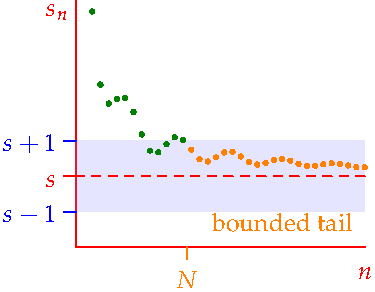
\includegraphics[scale=0.92]{convbdd}\par
	%\vspace{37.5pt}
	\vspace{12pt}
	\hfill\qedsymbol
\end{minipage}
\bigbreak

\goodbreak

The approach to part 2 is similar to part 1, we just need to be a bit cleverer to break up $\nm{s_nt_n-st}$.

\begin{proof}[Proof of Theorem \ref{thm:limitbasic}, part 2]
	Exercise \ref*{sec:limitdef}.\ref{exs:tbddproduct} deals with (and extends) the case when $s=0$. Instead suppose $s\neq 0$, and let $\epsilon>0$ be given. Since $s_n\to s$ and $t_n\to t$,
 	\begin{gather*}
 	(t_n)\text{ is bounded (Lemma)}:\exists M\text{ such that }\forall n, \nm{t_n}\le M\\
 	\exists N_1,N_2\text{ such that }n>N_1\implies \nm{s_n-s}<\frac\epsilon{2M}
 	\quad\text{and}\quad
	n>N_2\implies \nm{t_n-t}<\frac\epsilon{2\nm{s}}
 	\end{gather*}
 	Again let $N=\max\{N_1,N_2\}$, then
	\[
		\nm{s_nt_n-st}=\nm{s_nt_n-st_n+st_n-st} \overset{\smash{\triangle}}{\le}\nm{s_n-s}\nm{t_n}+\nm s\nm{t_n-t} < \frac\epsilon{2M}M+\nm s\frac\epsilon{2\nm s} =\epsilon\tag*{\qedhere}
	\]
\end{proof}

The proofs of parts 3 and 4 are in Exercise \ref{exs:limitlawsfinish}.



\boldinline{More basic examples}


With a few simple general examples, the limit laws allow us to rapidly compute the limits of a great variety of sequences.

\begin{thm}{}{limlaw2}
\exstart If $k>0$ then $\lim\frac 1{n^k}=0$
\begin{enumerate}\setcounter{enumi}{1}\itemsep0pt
	\item If $\nm a<1$ then $\lim a^n=0$
	\item If $a>0$ then $\lim a^{1/n}=1$
	\item $\lim n^{1/n}=1$
\end{enumerate}
\end{thm}


\begin{examples}{}{}
	\exstart $\displaystyle\lim (3n)^{2/n}=(\lim 3^{1/n})^2(\lim n^{1/n})^2=1$.
	\begin{enumerate}\setcounter{enumi}{1}
		\item $\displaystyle\lim\frac{n^{2/n}+\left(3-n^{-1}\sin n\right)^{1/5}}{4n^{-3/2}+7} =\frac{(\lim n^{1/n})^2 -\bigl(3-\lim\frac{\sin n}n\bigr)^{1/5}}{4\lim \frac 1{n^{3/2}}+7} =\frac{1-\sqrt[5]{3}}7$\par
		Note that $\lim\frac{\sin n}n=0$ follows from the squeeze theorem: $\nm{\frac{\sin n}n}\le \frac 1n\to 0$.
	\end{enumerate}
\end{examples}

%We give only a sketch proof: you should try to formalize these arguments as much as you can.

\begin{proof}
\begin{enumerate}
	\item This is Example \ref*{ex:moreeasylimits}.\ref{ex:stdzero}.
	\item The $a=0$ case is trivial. Otherwise, given $\epsilon>0$, let $N=\log_{\nm a}\epsilon$ and observe that
	\[n>N\implies \nm{a^n}<\nm{a^N}=\nm a^N=\epsilon\]
	\item Suppose $a\ge 1$, and let $s_n:=a^{1/n}-1$. Since $s_n>0$, the binomial theorem\footnotemark{} shows that
	\[a=(1+s_n)^n\ge 1+ns_n\implies 0<s_n\le\frac{a-1}n\]
	The squeeze theorem (\ref{thm:squeeze}) shows that $s_n\to 0$, whence $\lim a^{1/n}=1$.\par
	We leave the $a<1$ case and part 4 to Exercise \ref{exs:nrootlimit}. \hfill\qedhere
\end{enumerate}
\end{proof}

\vspace{-10pt}

\footnotetext{$(1+x)^n=\sum\limits_{k=0}^n\binom nk x^k=1+nx+\frac{n(n-1)}2x^2 + \frac{n(n-1)(n-2)}{2\cdot 3}x^3+\cdots +x^n$.}




\goodbreak



\boldsubsubsection{Divergence to $\pm\infty$ and the `divergence laws'}

We now consider unbounded sequences and provide a positive definition of a type of divergence.

\begin{defn}{}{diverge}
	We say that $(s_n)$ \emph{diverges to $\infty$} if,
	\[\forall M>0,\ \exists N\text{ such that }n>N\implies s_n>M\]
	We write $s_n\to\infty$ or $\lim s_n=\infty$. The definition for $s_n\to-\infty$ is similar.\smallbreak
	If $(s_n)$ neither converges nor diverges to $\pm\infty$, we say that it \emph{diverges by oscillation}.\footnotemark
\end{defn}

\footnotetext{In such cases $\lim s_n$ is meaningless; you likely wrote $\lim s_n=\text{DNE}$ (``does not exist'') in elementary calculus.}

Consider how $M$ is trying to describe ``closeness'' to infinity similarly to how $\epsilon$ measures closeness to $s$ in the original definition of limit (\ref{defn:limit}). 

\begin{examples}{}{}
	As with convergence proofs, it is a good idea to try some scratch work first!
	\begin{enumerate}
	  \item We show that $\lim (n^2+4n)=\infty$.\par
	  Let $M>0$ be given, and let $N=\sqrt M$. Then
		\[n>N\implies n^2+4n>n^2>N^2=M\]
	
		\item Prove that $s_n=n^5\textcolor{red}{-n^4-2n}+1\to\infty$.\par
		The \textcolor{red}{negative terms} cause some trouble, though our solution should be familiar from previous calculations:  
		\[s_n>\frac 12n^5\iff n^5>2(n^4+2n-1)\iff n>2+\frac 4{n^3}-\frac 1{n^4}\]
		Certainly this holds if $n>6$. We can now complete the proof.\par
		Let $M>0$ be given, and let $N=\max\{6,\sqrt[5]{2M}\}$. Then
		\[n>N\implies s_n>\frac 12n^5 >\frac 12(2M)=M\]
		
		\item Prove that the sequence defined by $s_n=n^2-n^3$ diverges to $-\infty$.\par
		First observe that
		\[s_n=n^2(1-n)<-\frac 12n^3\iff 1-n<-\frac 12n\iff n\ge 2\]
		Now let $M>0$ be given,\footnotemark{} and define $N=\max\{2,\sqrt[3]{2M}\}$. Then
		\[n>N\implies n>2\implies s_n<-\frac 12n^3<-\frac 12N^3\le -M\]
	\end{enumerate}
\end{examples}

\vspace{-13pt}

\footnotetext{The notion that $s_n\to-\infty$ can be phrased in multiple ways: some prefer
		\[\forall m<0,\ \exists N\text{ such that }n>N\implies s_n<m \tag{in our argument $M=-m$}\]
}

\goodbreak


Several of the limit laws can be adapted to sequences which diverge to $\pm\infty$.

\begin{thm}{}{divlaws}
	Suppose $\lim s_n=\infty$.
	\begin{enumerate}
		\item\label{thm:divlaws1} If $t_n\ge s_n$ for all (large) $n$, then $\lim t_n=\infty$
		\item If $\lim t_n$ exists and is \emph{finite}, then $\lim s_n+t_n=\infty$.
		\item If $\lim t_n>0$ then $\lim s_nt_n=\infty$.
		\item $\smash[b]{\lim\dfrac 1{s_n}=0}$
		\item If $\lim t_n=0$ and $t_n>0$ for all (large) $n$, then $\lim\dfrac 1{t_n}=\infty$
	\end{enumerate}
	Similar statements when $s_n\to-\infty$ should be clear.
\end{thm}

\begin{proof}
	We prove two of the results: try the rest yourself.
	\begin{enumerate}
		\item[2.] Since $(t_n)$ converges, it is bounded (below): $\exists m$ such that $\forall n,\ t_n\ge m$. Let $M$ be given. Since $\lim s_n=\infty$, $\exists N$ such that
		\begin{align*}
		n>N&\implies s_n>M-m \implies s_n+t_n>M-m+m=M
		\end{align*}
		\item[4.] Let $\epsilon>0$ be given, and let $M=\frac 1\epsilon$. Then $\exists N$ such that
		\[n>N\implies s_n>M=\frac 1\epsilon\implies \frac 1{s_n}<\epsilon\tag*{\qedhere}\]
	\end{enumerate}
\end{proof}

\boldinline{Rational Sequences}

We can now find the limit of any rational sequence: $\frac{p_n}{q_n}$ where $(p_n)$, $(q_n)$ are polynomials in $n$.

\begin{example}{}{}
	By applying Theorem \ref{thm:divlaws} (part 3) to
	\[s_n:=3n+4n^{-2}\to\infty\quad \text{and}\quad t_n=\frac 1{2-n^{-2}}\to\frac 12\]
	we see that
	\[\lim\frac{3n^3+4}{2n^2-1}=\lim\frac{3n+4n^{-2}}{2-n^{-2}}=\lim(3n+4n^{-2})\cdot\lim \frac 1{2-n^{-2}} =\infty\]
\end{example}

Indeed, you should be able to confirm the familiar result from elementary calculus:

\begin{cor}{}{}
	If $p_n,q_n$ are polynomials in $n$ with leading coefficients $p,q$ respectively then
	\[\lim\frac{p_n}{q_n}=\begin{cases}
	0&\text{if $\operatorname{deg}(p_n)<\operatorname{deg}(q_n)$}\\
	\dfrac pq&\text{if $\operatorname{deg}(p_n)=\operatorname{deg}(q_n)$}\\
	\sgn(\frac pq)\infty&\text{if $\operatorname{deg}(p_n)>\operatorname{deg}(q_n)$}
	\end{cases}\]
\end{cor}

\goodbreak


\begin{exercises}{}{}
	\emph{Key concepts/results:\quad ????}
 
	\begin{enumerate}
		\item%[2.]
		Suppose $\lim x_n=3$, $\lim y_n=7$ and that all $y_n$ are non-zero. Determine the following:
	  \begin{enumerate}
	    \item $\lim(x_n+y_n)$\qquad (b) \ $\lim\frac{3y_n-x_n}{y_n^2}$ \qquad (c) \ $\lim \sqrt{x_ny_n+4}$
	  \end{enumerate}
	  
	  
	  \item Consider $s_n=(100n)^{\frac{100}n}$. Describe $s_1$ (1 followed by how many zeros?). Repeat for $s_{10}$. Now compute the limit $\lim s_n$.
	  
	  
	  \item%[4.]
	  Define $(s_n)$ inductively via $s_1=1$ and $s_{n+1}=\sqrt{s_n+1}$ for $n\ge 1$.
	  \begin{enumerate}
		  \item List the first four terms of $(s_n)$.
		  \item It turns out that $(s_n)$ converges. Assume this and prove that $\lim s_n=\frac 12(1+\sqrt 5)$.
	  \end{enumerate}
	  
	  
	  \item Prove the following:
	  \begin{enumerate}
	    \item $\lim(n^3-98n)=\infty$\qquad\qquad (b) \ $\lim \bigl(\sqrt n-n+\frac 4n\bigr)=-\infty$
	  \end{enumerate}
	  
	  
	  \item%[6.]
	  Let $x_1=1$ and $x_{n+1}=3x_n^2$ for $n\ge 1$.
	  \begin{enumerate}
		  \item Show that if $(x_n)$ converges with limit $a$, then $a=\frac 13$ or $a=0$.
		  \item What is $\lim x_n$? Prove your assertion and explain what is going on.
	  \end{enumerate}
	  
	
		\item\label{exs:limitlawsfinish} We prove parts 3 and 4 of the limit laws (Theorem \ref{thm:limitbasic}). Assume $\lim s_n= s$ and $\lim t_n=t$.
		\begin{enumerate}
		  \item Suppose $t\neq 0$. Explain why $\exists N_1$ such that $n>N_1\implies \nm{t_n}>\frac 12\nm t$.
		  \item Let $\epsilon>0$ be given. Since $t_n\to t$, $\exists N_2$ such that $n>N_2\implies \nm{t_n-t}<\frac 12\nm t^2\epsilon$. Combine $N_1$ and $N_2$ to provide a proof that $\lim\frac 1{t_n}=\frac 1t$.
		  \item Explain how to conclude part 3: $\lim\frac{s_n}{t_n}=\frac st$.
		  \item Use the following inequality (valid when $s_n,s>0$) to help construct a proof for part 4
			\[\nm{s_n^{1/k}-s^{1/k}}=\frac{\nm{s_n-s}}{{s_n^{\frac{k-1}k}+s_n^{\frac{k-2}k}s^{\frac 1k}+\cdots +s^{\frac{k-1}k}}}\le \frac{\nm{s_n-s}}{s^{\frac{k-1}k}}\]
	 	\end{enumerate}
	
	
			\item\label{exs:nrootlimit}
			We finish the proof of Theorem \ref{thm:limlaw2}.
			\begin{enumerate}
			  \item Suppose $0<a<1$. Prove that $\lim a^{1/n}=1$.\par
				(\emph{Hint: consider $b=\frac 1a$\ldots})
				\item Let $s_n=n^{1/n}-1$. Apply the binomial theorem to $n=(1+s_n)^n$ to prove that $s_n<\sqrt{\frac 2{n-1}}$.
				Hence conclude that $\lim n^{1/n}=1$.
			\end{enumerate}
			
			
			\item Prove the remaining parts of Theorem \ref{thm:divlaws}.
			
			
			\item%[12.]
	  	Assume $s_n\neq 0$ for all $n$, and that the limit $L=\lim\smash[b]{\nm{\frac{s_{n+1}}{s_n}}}$ exists.
	  	\begin{enumerate}
		  	\item Show that if $L<1$, then $\lim s_n=0$.\par
		  	(\emph{Hint: if $L<a<1$, obtain $N$ so that $n>N\implies\nm{s_n}<a^{n-N}\nm{s_N}$})
		  	\item Show that if $L>1$, then $\lim\nm{s_n}=+\infty$.\par
		  	(\emph{Hint: apply (a) to the sequence $t_n=\frac 1{\nm{s_n}}$})
		  	\item%[14]
		  	Let $p>0$ and $a\in\R$ be given. How does $\lim\limits_{n\to\infty}\frac{a^n}{n^p}$ depend on the value of $a$?
	  \end{enumerate}

	\end{enumerate}
\end{exercises}

\clearpage



\subsection{Monotone and Cauchy Sequences}\label{sec:monocauchy}

The definition of limit (Definition \ref{defn:limit}) exhibits a major weakness; to demonstrate the convergence of a sequence, we must already know its limit! What we'd like is a method for determining whether a sequence converges \emph{without} first guessing a suitable limit.\footnote{This gets at the typical role of sequences in analysis: to demonstrate the existence of and define a new object (the limit) and, more broadly, to transfer useful properties from the sequence to the limit. For instance, if $(f_n)$ is a sequence of differentiable functions, we'd like to know if $\lim f_n(x)$ exists and is itself differentiable with derivative $\lim f_n'(x)$: discussions of this ilk will dominate Math 140B.} In this section we consider two important classes of sequence for which this can be done.

\begin{defn}{}{}
	A sequence $(s_n)$ is:
	\begin{itemize}
	  \item \emph{Monotone-up\footnotemark} if $s_{n+1}\ge s_n$ for all $n$.
		\item \emph{Monotone-down} if $s_{n+1}\le s_n$ for all $n$.
		\item \emph{Monotone} if either of the above is true.
	\end{itemize}
\end{defn}

\footnotetext{Some authors describe such as sequence as either \emph{non-decreasing} or \emph{increasing.} We prefer \emph{monotone-up/down} since this directly describes the direction of any potential movement in the sequence and prevents confusion over whether the inequality is strict. A sequence with $s_{n+1}>s_n$ may be described as \emph{strictly increasing} or \emph{strictly monotone-up.}}

\begin{examples}{}{}
	\exstart The sequence with $n\th$ term $s_n=\frac 7n+4$ is (strictly) monotone-down:
	\[s_{n+1}=\frac 7{n+1}<\frac 7n=s_n\]
	\begin{enumerate}\setcounter{enumi}{1}
	  \item A constant sequence $(s_n)=(s,s,s,s,\ldots)$ is \emph{both} monotone-up and monotone-down.
	\end{enumerate}
\end{examples}


\begin{thm}[lower separated=false, sidebyside, sidebyside align=top seam, sidebyside gap=0pt, righthand width=0.48\linewidth]{Monotone Convergence}{monotoneconv}\par
	Every bounded monotone sequence is convergent.\par Specifically:
	\begin{itemize}
	  \item If $(s_n)$ is bounded above and monotone-up, then $\lim s_n$ exists and equals $\sup\{s_n\}$.
	  \item If $(s_n)$ is bounded below and monotone-down, then $\lim s_n$ exists and equals $\inf\{s_n\}$.
	\end{itemize}
	\tcblower
	\flushright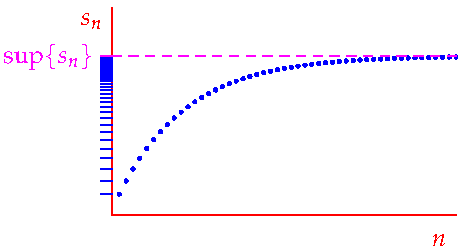
\includegraphics{monotone}
\end{thm}

In fact the conclusion $\lim s_n=\sup\{s_n\}$ holds for all monotone-up sequences: if unbounded above, then the result is $\infty$ (see Exercise \ref{exs:unbddmonotone}). The statement is $\lim s_n=\inf\{s_n\}$ for monotone-down sequences.


\begin{proof}
	If $(s_n)$ is bounded above, then $s:=\sup\{s_n\}$ exists by the completeness axiom ($s$ is finite!).\par
	Let $\epsilon>0$ be given. By Lemma \ref{lemm:contrasup}, there exists some $s_N>s-\epsilon$. Since $(s_n)$ is monotone-up, we have
	\[n>N\implies s_n\ge s_N>s-\epsilon\implies 0\le s-s_n<\epsilon\implies \nm{s-s_n}<\epsilon\]
	The monotone-down case is similar.
\end{proof}



\begin{examples}{}{}
	\exstart Define $(s_n)$ via $s_n=1$ and $s_{n+1}=\frac 15(s_n+8)$:
	\[(s_n)=\bigl(1,1.8,1.96,1.992,1.9984,1.99968,\ldots\bigr)\]
	The sequence certainly appears to be monotone-up and converging to 2. We prove this: 
	\begin{enumerate}\setcounter{enumi}{1}
	  \item[]\begin{description}
    	\item[\normalfont\emph{Bounded above}:] $s_n<2\implies s_{n+1}<\frac 15\left[2+8\right]=2$. By induction, $(s_n)$ is bounded above by 2.
    	\item[\normalfont\emph{Monotone-up}:] $s_{n+1}-s_n=\frac 45\left[2-s_n\right]>0$ since $s_n<2$.  
    	\item[\normalfont\emph{Convergence}:] By monotone convergence, $s=\lim s_n$ exists. Now use the limit laws to find $s$:
  \[s=\lim s_{n+1}=\frac 15\left(\lim s_n+8\right)=\frac 15(s+8)\implies s=2\] 
  	\end{description}
  
  	\item (Example \ref*{ex:methodmeanex}.\ref{ex:methodmeanex2}, cont.)\lstsp Let $s_1=2$ and $s_{n+1}=\frac 12\bigl(s_n+\frac 2{s_n}\bigr)$.
  	\begin{description}
	    \item[\normalfont\emph{Bounded below}:] The sequence is plainly always positive and thus bounded below by zero.
	    \item[\normalfont\emph{Monotone-down}:] We first obtain an improved lower bound:
	    \[s_{n+1}^2=\frac 14\left(s_n+\frac 2{s_n}\right)^2=2+\frac 14\left(s_n-\frac 2{s_n}\right)^2\ge 2\]
	    shows\footnotemark{} that $s_n^2\ge 2$ for all $n$. It follows that
	    \[\frac{s_{n+1}}{s_n}=\frac 12\left(1+\frac 2{s_n^2}\right)\le 1\implies s_{n+1}\le s_n\]
	    \item[\normalfont\emph{Convergence}:] By monotone convergence, $s=\lim s_n$ exists. Example \ref*{ex:methodmeanex}.\ref{ex:methodmeanex2} provides the limit:
	  	\[s=\frac 12\left(s+\frac 2s\right)\implies s=\sqrt 2\] 
  	\end{description}
  	This shows the necessity of completeness: $(s_n)$ is a monotone, bounded sequence of \emph{rational} numbers, but its limit is \emph{irrational.}
  	
  	\item A \emph{decimal} $0.d_1d_2d_3\ldots$ may be viewed as the limit of a monotone-up sequence of \emph{rational numbers}:
  	\[0.d_1d_2d_3\ldots =\lim_{n\to\infty}\sum_{k=0}^n \frac{d_k}{10^k}\]
  	This is bounded above by 1 and so converges. Compare this with Example \ref{ex:qsqqrt2nomax}.
  
    \item The sequence with $s_n=\left(1+\frac 1n\right)^n$ is particularly famous. In Exercise \ref{exs:edefn} we show that $(s_n)$ is monotone-up and bounded above. The limit provides, arguably, the oldest definition of $e$:
  	\[e:=\lim\left(1+\frac 1n\right)^n\]
  	%[(n,((1+1/n)^n).n()) for n in range(1,100)]} in Sage
	\end{enumerate}
\end{examples}

\vspace{-8pt}

\footnotetext{In case you've seen it before, this is the famous AM--GM inequality $\frac{x+y}2\ge \sqrt{xy}$ with $x=s_n$ and $y=\frac 2{s_n}$.}

\goodbreak



\boldsubsubsection{Limits Superior and Inferior}

One interpretation of $\lim s_n$ is that it approximately describes $s_n$ for large $n$. Even when a sequence does not have a limit, it remains useful to be able to describe its long-term behavior.


\begin{defn}{}{}
	Let $(s_n)$ be a sequence and define two related sequences $(v_N)$ and $(u_N)$:\par
	\begin{minipage}[t]{0.6\linewidth}\vspace{-12pt}
	\[\textcolor{blue}{v_N:=\sup\{s_n:n>N\}},\qquad \textcolor{Green}{u_N:=\inf\{s_n:n>N\}}\]
	\begin{enumerate}
	  \item The \emph{limit superior} of $(s_n)$ is
	  \[\limsup s_n=\begin{cases}
	  \lim\limits_{N\to\infty}\!v_N\!\!&\text{if $(s_n)$ bounded above}\\
	  \infty&\text{if $(s_n)$ unbounded above}
	  \end{cases}\]
	  \item The \emph{limit inferior} of $(s_n)$ is
	  \[\liminf s_n=\begin{cases}
	  \lim\limits_{N\to\infty}\!u_N\!\!&\text{if $(s_n)$ bounded below}\\
	  -\infty&\text{if $(s_n)$ unbounded below}
	  \end{cases}\]
	\end{enumerate}
	\end{minipage}
	\hfill
	\begin{minipage}[t]{0.39\linewidth}\vspace{-3pt}
		\hfill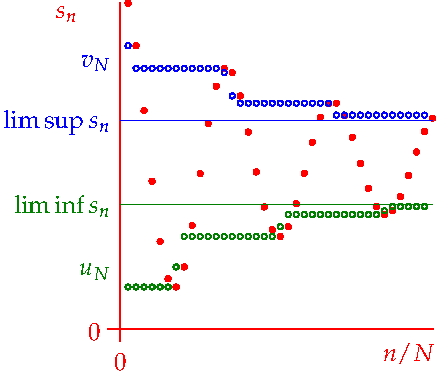
\includegraphics[scale=0.89]{limsup5}
	\end{minipage}
\end{defn}

The original sequence $\textcolor{red}{(s_n)}$ is \emph{almost} wedged between\footnote{A minor redefinition would remove the `almost,' but at the cost of making some subsequent arguments a little messier. It is still reasonable to think of $(u_N)$ and $(v_N)$ as providing a long-term envelope for the original sequence.} $\textcolor{blue}{(v_n)}$ and $\textcolor{Green}{(u_n)}$ in a situation reminiscent of the squeeze theorem (except $\limsup$ and $\liminf$ need not be equal). The next result summarizes the situation more formally; we omit the proof since these claims should be clear from the definition and previous results, particularly the monotone convergence theorem.


\begin{lemm}{}{limsupinf}
	\exstart $(v_N)$ is monotone-down, $(u_N)$ is monotone-up, and $u_N\le s_{N+1}\le v_N$.
	\begin{enumerate}\setcounter{enumi}{1}
	  \item\label{lemm:limsupinf1} $\limsup s_n$ and $\liminf s_n$ exist for any sequence (they might be infinite).
	  \item $\liminf s_n\le\limsup s_n$.
	\end{enumerate}
\end{lemm}



% \begin{proof}
% \begin{enumerate}
%		\item We are deleting successive terms from a set so $\sup$ is monotone-down, etc. Moreover $\inf\le \sup$ since these are of non-empty sets.
%   \item We deal only with $\limsup s_n$. There are several cases:
%   \begin{description}
% 	\item[$(s_n)$ unbounded above:] Then $\limsup s_n=\infty$. 
% 	\item[$(s_n)$ bounded above:] $(v_N)$ is a genuine sequence of real numbers which is \emph{monotone-down.} We either have
% 	\begin{itemize}
% 	  \item $(v_N)$ bounded below, in which case it converges by Theorem \ref{thm:monotoneconv}.
% 	  \item $(v_N)$ unbounded below, in which case $\limsup s_n=-\infty$.
% 	\end{itemize}
% \end{description}
% 	\item This is trivial since $u_N\le v_N$ for all $N$.\hfill\qedhere
% \end{enumerate}
% \end{proof}

\begin{examples}{}{limsupexs}
	\exstart The picture shows sequences $\textcolor{red}{(s_n)}$, $\textcolor{Green}{(u_N)}$ and $\textcolor{blue}{(v_N)}$ when $s_n=6+(-1)^n\left(1+\frac 5n\right)$
	\begin{enumerate}\setcounter{enumi}{1}
		\begin{minipage}[t]{0.52\linewidth}\vspace{-8pt}
			\item[]We won't compute everything precisely, but the picture suggests $\textcolor{red}{(s_n)}$ has two ``sub"sequences: the odd terms increase while the even terms decrease towards, respectively
			\[\textcolor{Green}{\liminf s_n=5},\qquad \textcolor{blue}{\limsup s_n=7}\]
			Here is one value from each derived sequence:
			\begin{gather*}
				\textcolor{Green}{u_3}=\inf\{s_n:n>3\}=\textcolor{red}{s_5}=4\\
				\textcolor{blue}{v_7}=\sup\{s_n:n>7\}=\textcolor{red}{s_8}=7.625
			\end{gather*}
		\end{minipage}
		\hfill
		\begin{minipage}[t]{0.47\linewidth}\vspace{-8pt}
			\flushright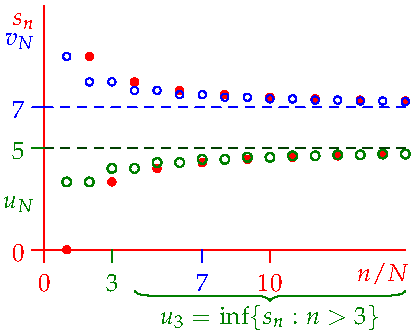
\includegraphics[scale=0.9]{limsup4}
		\end{minipage}
	
		
		\item If $s_n=\frac 1n$, then $v_N=s_{N+1}$ and $u_N=0$ for all $N$, whence $\limsup s_n=\liminf s_n=0$.
	
		\item Let $s_n=(-1)^n$. This time the calculation is easy:
		\[u_N=\inf\{s_n:n>N\}=-1\quad\text{and}\quad v_N=\sup\{s_n:n>N\}=1\]
		Therefore $\limsup s_n=1$ and $\liminf s_n=-1$.
	\end{enumerate}
	
\end{examples}


\begin{lemm}[lower separated=false, sidebyside, sidebyside align=top seam, sidebyside gap=0pt, righthand width=0.48\linewidth]{}{limbig}
	For any sequence $(s_n)$,
	\[\liminf s_n=\limsup s_n \implies\lim s_n\text{ exists}\]
	(the limit can be infinite!).\smallbreak
	In such a case all three values are equal.
	\tcblower
	\hfill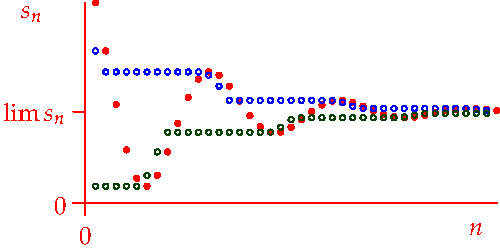
\includegraphics[scale=0.8]{limsup1}
\end{lemm}

In fact the converse to this is also true: we could prove it now, but it will come for free a little later\ldots


\begin{proof}
		\begin{description}
			\item[\normalfont($s$ finite)\lstsp] Since $u_{n-1}\le s_n\le v_{n-1}$ for all $n$, the squeeze theorem tells us that $\lim s_n=s$.
			\item[\normalfont($s=\infty$)\lstsp] Since $u_{n-1}\le s_n$ for all $n$ and $\lim u_{n-1}=\infty$, it follows (Theorem \ref*{thm:divlaws}.\ref{thm:divlaws1}) that $\lim s_n=\infty$.
			\item[\normalfont($s=-\infty$)\lstsp] This time $s_n\le v_{n-1}\to-\infty\implies\lim s_n=-\infty$.\qedhere
		\end{description}

% 	\begin{itemize}
% 	  \item[$(\Rightarrow)$] Suppose $\limsup s_n=\liminf s_n=s$. There are three cases.
% 		\begin{description}
% 			\item[\normalfont($s$ finite)\lstsp] Since $u_{n-1}\le s_n\le v_{n-1}$ for all $n$, the squeeze theorem tells us that $\lim s_n=s$.
% 			\item[\normalfont($s=\infty$)\lstsp] Since $u_{n-1}\le s_n$ for all $n$ and $\lim u_{n-1}=\infty$, it follows (Theorem \ref*{thm:divlaws}.\ref{thm:divlaws1}) that $\lim s_n=\infty$.
% 			\item[\normalfont($s=-\infty$)\lstsp] This time $s_n\le v_{n-1}\to-\infty\implies\lim s_n=-\infty$.
% 		\end{description}
% 	
% 		\item[$(\Leftarrow)$] Let $\lim s_n=s$. We have the same three cases.
% 		\begin{description}
% 			\item[\normalfont($s$ finite)\lstsp] Since $\lim s_N=s$, the definition of limit says that,
% 			\[\forall\epsilon>0,\ \exists \widetilde N\text{ such that }n>\widetilde N\implies \nm{s_n-s}<\epsilon \implies s-\epsilon< s_n<s+\epsilon\]
% 			Taking the supremum and then the limit, we see that
% 			\begin{align*}
% 				N\ge \widetilde N&\implies v_N=\sup\{s_n:n>N\}\le s+\epsilon\\
% 				&\implies \limsup s_n=\lim_{N\to\infty}v_N\le s+\epsilon\tag*{(Theorem \ref{thm:limitgreatk})}
% 			\end{align*}
% 			We see similarly that
% 			\begin{align*}
% 				N\ge \widetilde N&\implies u_N=\inf\{s_n:n>N\}\ge s-\epsilon\\
% 				&\implies \liminf s_n=\lim_{N\to\infty}u_N\ge s-\epsilon
% 			\end{align*}
% 			Since these hold for every $\epsilon>0$ we conclude that $\limsup s_n\le s\le\liminf s_n$ (!).\smallbreak
% 			Combining with Lemma \ref{lemm:limsupinf} ($\liminf s_n\le\limsup s_n$) we see that all three terms are equal.
% 			\item[\normalfont($s=\infty$)\lstsp] Since $\lim s_n=\infty$, we have
% 			\begin{align*}
% 			\forall M>0,\ \exists N\text{ such that }n>N&\implies s_n>M\\
% 			&\implies u_N=\inf\{s_n:n>N\}\ge M
% 			\end{align*}
% 			That is, $\liminf s_n=\lim u_N=\infty$. Plainly $\limsup s_n\ge\liminf s_n=\infty$ also.
% 			\item[\normalfont($s=-\infty$)\lstsp] $\lim s_n=-\infty$ is similar to the previous case.\hfill\qedhere
% 		\end{description}
% 	\end{itemize}
\end{proof}

\goodbreak



\boldsubsubsection{Cauchy Sequences}

We now come to a class of sequences whose analogues will dominate your study of analysis.

\begin{defn}{}{cauchy}
A sequence $(s_n)$ is \emph{Cauchy\footnotemark} if
\[\forall\epsilon>0,\ \exists N\ \text{such that}\  m,n>N\implies\nm{s_n-s_m}<\epsilon\]
\end{defn}

\footnotetext{Augustin-Louis Cauchy (1789--1857) was a French mathematician, responsible (in part) for the $\epsilon$-$N$ definition of limit.}

A sequence is Cauchy when terms in the tails of the sequence are constrained to stay close to one another. As we'll see shortly, this will provide an alternative way to detect and describe \emph{convergence.}


\begin{examples}{}{cauchy}
	\exstart Let $s_n=\frac 1n$. Let $\epsilon>0$ be given and let $N=\frac 1\epsilon$. Then\footnotemark
	\[m>n>N\implies \nm{s_m-s_n}=\frac 1n-\frac 1m<\frac 1n<\frac 1N=\epsilon\]
	Thus $(s_n)$ is Cauchy. A similar argument works for any $s_n=\frac 1{n^k}$ for positive $k$.
	  
	\begin{enumerate}\setcounter{enumi}{1}
	  \item\label{ex:cauchy3} Suppose $s_1=5$ and $s_{n+1}=s_n+\frac{1}{n(n+1)}$. As before, let $\epsilon>0$ be given and let $N=\frac 1\epsilon$. Then,
	  \begin{align*}
	  &\nm{s_{n+1}-s_n}=\frac 1{n(n+1)}=\frac 1n-\frac 1{n+1}\\
	  \implies &\nm{s_m-s_n}\overset{\triangle}{\le} \nm{s_{n+1}-s_n}+\cdots+\nm{s_m-s_{m-1}} = \frac 1n-\frac 1m<\frac 1n<\frac 1N=\epsilon
	  \end{align*}
	  Again we have a Cauchy sequence.
	  
	  \goodbreak
	  
	  
	  \begin{minipage}[t]{0.5\linewidth}\vspace{0pt}
		  \item\label{ex:cauchy2} Define $(s_n)_{n=0}^\infty$ inductively:
		  \begin{gather*}
		  	s_0=1,\quad s_{n+1}=
		  	\begin{cases}
		  		s_n+3^{-n}&\text{if $n$ even}\\
		  		s_n-2^{-n}&\text{if $n$ odd}
		  	\end{cases}
		  	\\[5pt]
		  	(s_n)=\left(1,2,\frac 32,\frac{29}{18},\frac{107}{72},\ldots\right)
		  \end{gather*}
	  	Since $\nm{s_{n+1}-s_n}\le 2^{-n}$, we see that\vspace{-3pt}
	  \end{minipage}
	  \hfill
	  \begin{minipage}[t]{0.49\linewidth}\vspace{-5pt}
	  	\hfill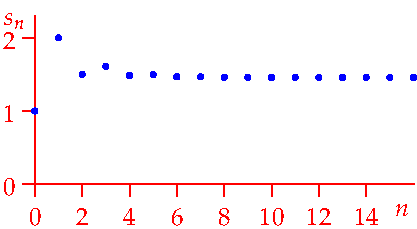
\includegraphics{cauchyex}
	  \end{minipage}\par\vspace{-8pt}
  	\begin{align*}
  		m>n\implies \nm{s_m-s_n}&\overset{\smash{\triangle}}{\le} \nm{s_{n+1}-s_n}+\cdots+\nm{s_m-s_{m-1}} =\sum_{k=n}^{m-1}\nm{s_{k+1}-s_k}\\
  		&\le \sum_{k=n}^{m-1}2^{-k} =\frac{2^{-n}-2^{-m}}{1-2^{-1}}<2^{1-n}
  	\end{align*}
  	where we used the familiar geometric sum formula from calculus: $\smash{\sum\limits_{k=a}^{b-1} r^k=\frac{r^a-r^{b}}{1-r}}$.\par
  	Suppose $\epsilon>0$ is given, and let $N=1-\log_2\epsilon =\log_2\frac 2\epsilon$. Then
 	 	\[
 	 		m>n>N\implies \nm{s_m-s_n}<2^{1-n} <2^{1-N}=\epsilon
 	 	\]
  	We conclude that $(s_n)$ is Cauchy.
	\end{enumerate}
\end{examples}

\footnotetext{Since $m,n$ are arbitrary, WLOG we may assume $m>n$; equality is never interesting in these situations. This assumption is very common and we'll use it repeatedly without comment.}

The picture in the last example illustrates the essential point regarding Cauchy sequences: $(s_n)$ appears very much to converge\ldots


%Another example: $s_{n+1}=s_n+\frac{\sin n}{n(n+1)}$ has $\nm{s_{n+1}-s_n}=\frac 1n-\frac 1{n+1}\implies \nm{s_m-s_n}\le \frac 1n-\frac 1m<\frac 1n<\frac 1N=\epsilon$

\goodbreak



\begin{thm}{Cauchy Completeness}{convcauchy}
	A sequence of real numbers is convergent if and only if it is Cauchy.
\end{thm}

\begin{proof}
	\begin{description}
		\item[$(\Rightarrow)$] Suppose $\lim s_n=s$ (finite). Given $\epsilon>0$ we may choose $N$ such that
		\begin{align*}
			m,n>N&\implies \nm{s_n-s}<\frac\epsilon 2\quad\text{and}\quad\nm{s_m-s}<\frac\epsilon 2\\
			&\implies\nm{s_n-s_m}=\nm{s_n-s+s-s_m}\overset{\smash{\triangle}}{\le}\nm{s_n-s}+\nm{s-s_m}<\epsilon
		\end{align*}
		whence $(s_n)$ is Cauchy.
		
		\item[$(\Leftarrow)$] To discuss the convergence of $(s_n)$ we first need a potential limit! In view of Lemma \ref{lemm:limbig}, the obvious candidates are $\limsup s_n$ and $\liminf s_n$. We have two goals: show that $(s_n)$ is bounded whence the limits superior and inferior are \emph{finite}; then show that these are \emph{equal.}
		\begin{description}
			\item[\normalfont(Boundedness of $(s_n)$)] Take $\epsilon=1$ in Definition \ref{defn:cauchy}:
			\[\exists N\text{ such that }m,n>N\implies\nm{s_n-s_m}<1\]
			It follows that
			\[n>N\implies\nm{s_n-s_{N+1}}<1\implies s_{N+1}-1<s_n<s_{N+1}+1\]
			whence $(s_n)$ is bounded; it follows that $\limsup s_n$ and $\liminf s_n$ are \emph{finite.}
			
			\goodbreak
			
			\item[\normalfont($\limsup s_n=\liminf s_n$)] Since $(s_n)$ is Cauchy, given $\epsilon>0$,
			\[\exists N\text{ such that }m,n>N\implies \nm{s_n-s_m}<\epsilon\implies s_n<s_m+\epsilon\]
			Taking $v_N=\sup\{s_n:n>N\}$, we see that
			\begin{align*}
				m>N&\implies v_N\le s_m+\epsilon %\tag{since $v_N=\sup\{s_n:n>N\}$}%\\
				%&\implies v_N\le u_N+\epsilon \tag{since $u_N=\inf\{s_m:m>N\}$}
			\end{align*}
			Taking the infimum of the right hand side yields
			\begin{align*}
				%m>N&\implies v_N\le s_m+\epsilon \tag{since $v_N=\sup\{s_n:n>N\}$}\\
				&v_N\le u_N+\epsilon \tag{since $u_N=\inf\{s_m:m>N\}$}
			\end{align*}
			Since $(v_N)$ is monotone-down and $(u_N)$ monotone-up, we see that
			\[\limsup s_n\le v_N\le u_N+\epsilon\le\liminf s_n+\epsilon \implies \limsup s_n\le \liminf s_n+\epsilon \]
			This last holds for all $\epsilon>0$, whence $\limsup s_n\le \liminf s_n$. By Lemma \ref{lemm:limsupinf} we have equality.
		\end{description}

	By Lemma \ref{lemm:limbig}, we conclude that $(s_n)$ converges to $\limsup s_n=\liminf s_n$.\hfill\qedhere
\end{description}
\end{proof}


In view of the Theorem, the previous examples converge. All three limits can be found precisely (for instance, see Exercise \ref{exs:cauchygeomeval}). With a small modification to the second example, however, we obtain something genuinely new:

\begin{example*}{\ref*{ex:cauchy}.\ref{ex:cauchy3} cont}{}
Let $s_1=5$ and , for each $n$, define $s_{n+1}=s_n+\frac{\sin n}{n(n+1)}$. Since $\nm{\sin n}\le 1$, the computation proceeds almost the same as before:
\[\nm{s_{n+1}-s_n}=\frac{\nm{\sin n}}{n(n+1)}\le \frac 1{n(n+1)}=\cdots\]
The new sequence is Cauchy and therefore convergent; good luck explicitly finding its limit though!
\end{example*}

The main point is easy to miss: Cauchy Completeness provides a powerful tool for determining whether a sequence converges \emph{without first guessing a limit.} While the result depends on monotone convergence (via limit superior/inferior), it is more powerful in that it applies even to non-monotone sequences. We finish with an application of this idea.



\boldinline{An Alternative Definition of $\R$}

Cauchy sequences suggest a \emph{definition} of the real numbers which does not rely on Dedekind cuts (Section \ref{sec:dedekind}).\smallbreak
Define an equivalence relation $\sim$ on the collection $\cC$ of all Cauchy sequences of rational numbers:\footnote{We don't need real numbers to define the limit of the \emph{rational} sequence $(s_n-t_n)$: $\forall \epsilon\in\Q^+$ is enough\ldots}
\[(s_n)\sim(t_n)\iff \lim(s_n-t_n)=0\]
We then define $\R:=\quotient{\cC}{\sim}$. All this is done without reference to Cauchy Completeness, though it certainly informs our intuition that $(s_n)$ and $(t_n)$ have the same limit. Some work is still required to define $+,\cdot,\le$, etc., and to verify the axioms of a complete ordered field---we won't pursue this.

\goodbreak

% 
% \boldinline{Decimal Numbers}\phantomsection\label{ssec:decimals}
% 
% What is a decimal? It is clear what a \emph{terminating} decimal should mean since any such is a rational number; for instance
% \[12.31452=\frac{1231452}{10000}\]
% What about a non-terminating decimal? We can view such as the limit of a \emph{sequence of rational numbers}; for example
% \[3.14159\cdots =\lim s_n\text{ \ where \ } (s_n)=\left(3,\frac{31}{10},\frac{314}{100},\frac{3141}{1000},\ldots\right)\]
% Of course, we need to show that every such sequence converges!\smallbreak
% Given integers $d_k\in\{0,1,2,\ldots,9\}$, consider the sequence $(s_n)$ where
% \[s_n=0.d_1d_2\cdots d_n=\frac{d_1}{10}+\cdots+\frac{d_n}{10^n}=\sum_{k=1}^n\frac{d_k}{10^k}\]
% Certainly $(s_n)$ is a sequence of rational numbers. We prove that it is Cauchy:\smallbreak
% Let $\epsilon>0$ be given and choose $N=-\log_{10}\epsilon =\log_{10}\epsilon^{-1}$. Then
% \begin{align*}
% 	m>n>N\implies \nm{s_n-s_m} &=\sum_{k=n+1}^m 10^{-k}d_k \tag{$= 0.0\cdots 0d_{n+1}\cdots d_{m}$}\\
% 	&<10^{-n}<10^{-N}=\epsilon
% \end{align*}
% The sequence is Cauchy and thus converges\footnote{Since $s_n$ is plainly monotone-up and bounded above by 1, we could instead conclude this directly using the monotone convergence theorem.} to some \emph{real number} $s$. This limit is precisely what we mean by the decimal
% \[s=0.d_1d_2d_3\cdots\]
% The upshot is that every decimal expression represents a real number. We'll return to this example once we consider infinite series.

\goodbreak

\begin{exercises}{}{}
	\emph{Key concepts/results:\quad ????}

	\begin{enumerate}
	  \item Use Definition \ref{defn:cauchy} to show that the sequence with $s_n=\frac 1{n^2}$ is Cauchy. Repeat for $t_n=\frac 1{n(n-2)}$.
	  
	  \item%[9.]
	  Let $s_1=1$ and $s_{n+1}=\frac n{n+1}s_n^2$ for $n\ge 1$.
	  \begin{enumerate}
		  \item Find $s_2, s_3$ and $s_4$.
		  \item Show that $\lim s_n$ exists and hence prove that $\lim s_n=0$.
	  \end{enumerate}
	  
	  
	  \item%[10.]
	  Let $s_1=1$ and $s_{n+1}=\frac 13(s_n+1)$ for $n\ge 1$.
	  \begin{enumerate}
		  \item Find $s_2, s_3$ and $s_4$.
		  \item Use induction to show that $s_n>\frac 12$ for all $n$, and conclude that $(s_n)$ is monotone-down.
		  \item Show that $\lim s_n$ exists and find $\lim s_n$.
	  \end{enumerate}
	  
	  
	  \item%[6.]modified
	  \begin{enumerate}
	  	\item Let $(s_n)$ be a sequence such that $\forall n,\ \nm{s_{n+1}-s_n}\le 3^{-n}$. Prove that $(s_n)$ is Cauchy.
	  	\item Let $s_1=10$ and, for each $n$, let $s_{n+1}=s_n+\frac{\cos n}{3^n}$. Explain why $(s_n)$ is convergent.
	  	\item Is the result in (a) true if we only assume that $\nm{s_{n+1}-s_n}\le \frac 1n$ for all $n\in\N$?
	  \end{enumerate}
	  
	    
	  \item\label{exs:unbddmonotone} Suppose $(s_n)$ is \emph{unbounded} and monotone-up. Prove that $\lim s_n=\infty$.\par
	  (\emph{Thus $\lim s_n=\sup\{s_n\}$ for any monotone-up sequence}) 
	  
	
		\item Let $s_n=\frac{(-1)^n}n$. Find the sequences $(u_N),(v_N)$ and explicitly compute $\limsup s_n$ and $\liminf s_n$.
	  
	  
	  \item\label{exs:cauchygeomeval} Consider the sequence in Example \ref*{ex:cauchy}.\ref{ex:cauchy2}. Explain why $s_{2n}=s_{2n-2}-\frac 2{4^n}+\frac 9{9^n}$.\par
	  Now use the geometric sum formula to evaluate $\lim s_{2n}$.\par
	  (\emph{Since $(s_n)$ converges, this means the original sequence has the same limit})
	  
	  
	  \item%[7.]
	  Let $S$ be a bounded nonempty set for which $\sup S\notin S$. Prove that there exists a monotone-up sequence $(s_n)$ of points in $S$ such that $\lim s_n=\sup S$.\par
	  (\emph{Hint: for each $n$, use $\sup S-\frac 1n$ to build $s_n$})
	  
	  
	  \item%[8.]
	  Let $(s_n)$ be a monotone-up sequence of positive numbers and define $\sigma_n=\frac 1n(s_1+s_2+\cdots+s_n)$. Prove that $(\sigma_n)$ is monotone-up.
	
	  
	  
	  \item\label{exs:edefn} (Hard!)\lstsp We prove that the sequence defined by $s_n=\left(1+\frac 1n\right)^n$ is convergent.
	  \begin{enumerate}
	    \item Show that
	    \[\frac{1+\frac 1{n+1}}{1+\frac 1n}=1-\frac 1{(n+1)^2}\quad \text{and}\quad \frac{1+\frac 1n}{1+\frac 1{n+1}}=1+\frac 1{n(n+2)}\]
		  \item Prove \emph{Bernoulli's inequality} by induction.
		  \begin{quote}
		  	For all real $x>-1$ and $n\in\N_0$ we have $(1+x)^n\ge 1+nx$.
		  \end{quote}
			\item Use parts (a) and (b) to prove that $(s_n)$ is monotone-up.\par
			(\emph{Hint: consider $\frac{s_{n+1}}{s_n}$}) 
			\item Similarly, show that $t_n:=\left(1+\frac 1n\right)^{n+1} =\left(1+\frac 1n\right)s_n$ defines a monotone-down sequence.
			\item Prove that $(s_n)$ and $(t_n)$ converge, and to the \emph{same} limit (this limit is $e$).\par
			(\emph{Hint: compute $t_n-s_n$})
		\end{enumerate}
	  
	
	
	% \begin{enumerate}
	%   \item This is a simple induction: the induction step requires
	%   \begin{align*}
	%   (1+x)^{n+1}&=(1+x)^n(1+x)\ge(1+nx)(1+x)=1+(n+1)x+nx^2\\
	%   &\ge 1+(n+1)x
	%   \end{align*}
	%   \item Consider the quotient
	% 	\begin{align*}
	% 		\frac{l_{n+1}}{l_n}&=\frac{\left(1+\frac 1{n+1}\right)^{n+1}}{\left(1+\frac 1n\right)^n} =\left[\frac{n}{n+1}\right]^n\left[\frac{n+2}{n+1}\right]^{n+1} =\left[\frac{n(n+2)}{(n+1)^2}\right]^{n+1}\frac{n+1}n\\
	% 		&=\left[\frac{(n+1)^2-1}{(n+1)^2}\right]^{n+1}\frac{n+1}n =\left[1-\frac 1{(n+1)^2}\right]^{n+1}\frac{n+1}n\\
	% 		&\ge \left(1-\frac{n+1}{(n+1)^2}\right)\frac{n+1}n=1\tag*{(by part 1.)}
	% 	\end{align*}
	%   \item We again use Bernoulli's inequality:
	% 	\begin{align*}
	% 		\frac{u_{n+1}}{u_n}&=\frac{\left(1+\frac 1{n+1}\right)^{n+2}}{\left(1+\frac 1n\right)^{n+1}} =\left[\frac{n}{n+1}\right]^{n+1}\left[\frac{n+2}{n+1}\right]^{n+2} =\left[\frac{(n+1)^2}{n(n+2)}\right]^{-(n+2)}\frac{n+1}n\\
	% 		&=\left[\frac{n(n+2)+1}{n(n+2)}\right]^{-(n+2)}\frac{n+1}n =\frac 1{\left[1+\frac 1{n(n+2)}\right]^{n+2}}\frac{n+1}n\\
	% 		&\le \frac 1{1+\frac 1n}\cdot\frac{n+1}n=1\tag*{\qedhere}
	% 	\end{align*}
	% \end{enumerate}
	
	% Note that $u_n=(1+\frac 1n)l_n>l_n$ and that $(l_n)$ is non-decreasing and $u_n$ non-increasing. Thus $(l_n)$ is bounded above (by $u_1$ say). Similarly $(u_n)$ is bounded below. The monotone convergence theorem says that both sequences converge.\\
	% Moreover,
	% \[\nm{u_n-l_n}=\left[\left(1+\frac 1n\right)-1\right]\left(1+\frac 1n\right) =\frac 1nl_n\to 0\]
	% since $(l_n)$ is convergent, thus both sequences converge to the same limit.
	% \end{proof}
	
	
	\end{enumerate}
\end{exercises}

\clearpage


\subsection{Subsequences}\label{sec:subseq}

The general behavior of a sequence is often hard to ascertain, but if we delete some of its terms we might obtain a \emph{subsequence} with interesting behavior.

\begin{defn}{}{}
	Let $(s_n)$ be a sequence. A \emph{subsequence} $(s_{n_k})$ is a subset $(s_{n_k})\subseteq (s_n)$, where 
	\[n_1<n_2<n_3<\cdots\]
	A subsequence is simply an infinite subset, with order inherited from the original sequence.
\end{defn}

\begin{example}[lower separated=false, sidebyside, sidebyside align=top seam, sidebyside gap=0pt, righthand width=0.38\linewidth]{}{}
	Take $s_n=(-1)^n$ (recall Example \ref*{ex:divergenceeasy}.\ref{ex:divergenceeasy2}) and let $n_k=2k$. Then $\textcolor{blue}{s_{n_k}}=1$ for all $k$. Note two important facts:
	\begin{itemize}
	  \item The subsequence $(\textcolor{blue}{s_{n_k}})_{k=0}^\infty$ is indexed by $\textcolor{blue}{k}$, not $n$.
	  \item The subsequence is constant and thus \emph{convergent.}
	\end{itemize} 
	\tcblower
	\hfill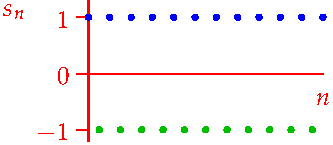
\includegraphics{divergent3}
\end{example}

Our main goal in this section is to prove the result illustrated in the example, that every bounded sequence has a convergent subsequence (the famous Bolzano--Weierstraß theorem).


\begin{lemm}{}{subseqconv}
	If $\lim\limits_{n\to\infty} s_n=s$, then every subsequence $(s_{n_k})$ also satisfies $\lim\limits_{k\to\infty} s_{n_k}=s$.\vspace{-3pt}
\end{lemm}

\begin{proof}
	Suppose $s$ is finite and let $\epsilon>0$ be given. Then $\exists N$ such that $n>N\implies \nm{s_n-s}<\epsilon$. Since $n_k\ge k$ for all $k$, we see that
	\[k>N\implies n_k>N\implies \nm{s_{n_k}-s}<\epsilon\]
	The case where $s=\pm\infty$ is an exercise.
\end{proof}

\begin{lemm}{}{monosub}
	Every sequence has a monotonic subsequence.
\end{lemm}

\begin{proof}
	Given $(s_n)$, we call the term $s_n$ `dominant' if $m>n\implies s_m<s_n$. There are two cases:
% 	\begin{minipage}[t]{0.6\linewidth}\vspace{0pt}
\begin{enumerate}\itemsep0pt
  \item If there are \textcolor{blue}{infinitely many dominant terms}, then the subsequence of such is \textcolor{blue}{monotone-down}. %Moreover if $s_n$ is dominant, then $v_{n-1}=\sup\{s_k:k>n-1\}=s_n$, whence the subsequence of dominant terms tends to $\limsup s_n$ (could be $-\infty!$).
  \item If there are \textcolor{magenta}{finitely many dominant terms}, choose $s_{n_1}$ after all such. Since $s_{n_1}$ is not dominant, $\exists n_2>n_1$ such that $s_{n_2}\ge s_{n_1}$. Induct to obtain a \textcolor{Green}{monotone-up} subsequence.
  \end{enumerate}
  
	\begin{center}
		\begin{tabular}{c@{\qquad}c}
	  	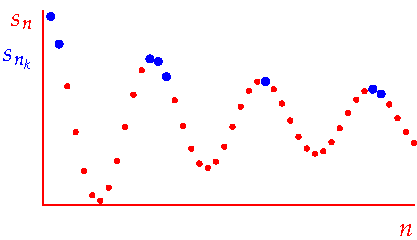
\includegraphics[scale=1]{dominant1}&
	  	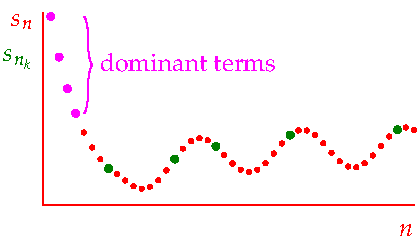
\includegraphics[scale=1]{dominant2}\\[-3pt]
	  	Case 1: \textcolor{blue}{monotone-down subsequence}&Case 2: \textcolor{Green}{monotone-up subsequence}
	  \end{tabular}\\[-8pt]
	  \hfill\qedhere
	\end{center}
\end{proof}


\goodbreak

\begin{thm}{}{subseqhard}
	Given a sequence $(s_n)$, there exist subsequences $(s_{n_k})$ and $(s_{n_l})$ such that
	\[\lim s_{n_k}=\limsup s_n\quad\text{and}\quad \lim s_{n_l}=\liminf s_n\]
	Combining with the lemmas, we may assume these subsequences are monotonic.
\end{thm}


\begin{example}[lower separated=false, sidebyside, sidebyside align=top seam, sidebyside gap=0pt, righthand width=0.47\linewidth]{}{subseqconv}
	The picture shows the sequence with $n\th$ term
	\[
		s_n=
		\begin{cases}
			\frac 4n(-1)^{\frac n2+1}&\text{when $n$ is even}\\
			1-\frac 1{n}&\text{when $n$ is odd}
		\end{cases}
	\]
	Monotonic subsequences with limits $\textcolor{blue}{\limsup s_n=1}$ and $\textcolor{Green}{\liminf s_n=0}$ are indicated.
	\tcblower
	\hfill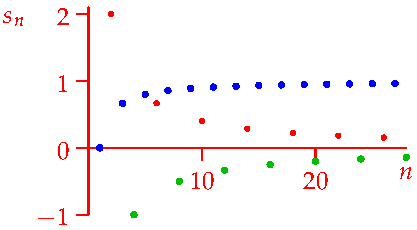
\includegraphics[scale=1]{exlimsupconv2}
\end{example}

\begin{proof}
	We prove only the $\limsup$ claim since the other is similar. There are three cases to consider; visualizing the third is particularly difficult and may take several readings.
	\begin{description}
	  \begin{minipage}[t]{0.56\linewidth}\vspace{-10pt}
		  \item[\normalfont ($\limsup s_n=\infty$)]\lstsp Since $(s_n)$ is unbounded above, for any $k>0$ there exist \emph{infinitely many} terms $s_n>k$. We may therefore inductively choose a subsequence $(\textcolor{blue}{s_{n_k}})$ via
		  \begin{gather*}
		  	n_1=\min\{n\in\N:s_{n_1}>1\}\\
		  	n_k=\min\{n\in\N:n_k>n_{k-1},\ s_{n_k}>k\}
		  \end{gather*}
		  Choosing the minimum isn't necessary here, but it at least keeps the subsequence explicit. Clearly
			\[s_{n_k}>k\implies \lim_{k\to\infty} s_{n_k}=\infty=\limsup s_n\]
	  \end{minipage}
	 	\hfill
	 	\begin{minipage}[t]{0.4\linewidth}\vspace{-10pt}
		  \hfill
		  \begin{tabular}{c@{}}
		  	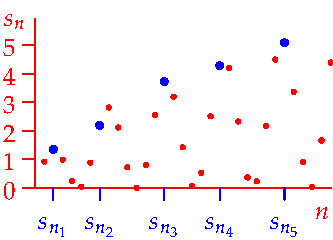
\includegraphics{dominant3}\\
		  	Example: $\limsup \frac{\sqrt n}2(1+\sin n)=\infty$
		  \end{tabular}
	  \end{minipage}
	  
		\item[\normalfont ($\limsup s_n=-\infty$)]\lstsp Since $\liminf s_n\le \limsup s_n=-\infty$, Lemma \ref{lemm:limbig} says that $\lim s_n=-\infty$, whence $(s_n)$ itself is a suitable subsequence.
		
	  \item[\normalfont ($\limsup s_n=v$ finite)]\lstsp We follow an inductive construction: let $n_1=1$ and define $s_{n_k}$ for $k\ge 2$ via,
		\begin{itemize}
		  \item Since $(v_N)$ is monotone-down and converges to $v$, take $\epsilon=\frac 1{2k}$ to see that\footnotemark{}
		  \[\exists N_k\ge n_{k-1}\text{ such that }v\le v_{N_k}<v+\frac 1{2k}\]
	
		  \item Since $v_{N_k}=\sup\{s_n:n>N_k\}$, Lemma \ref{lemm:contrasup} says
		  \[\exists n_k>N_k\text{ such that }s_{n_k}>v_{N_k}-\frac 1{2k}\]
		\end{itemize}
		But then $\nm{v-s_{n_k}}\overset{\smash{\triangle}}{\le}\nm{v-v_{N_k}}+\nm{v_{N_k}-s_{n_k}}<\frac 1k$. The squeeze theorem says that $\lim\limits_{k\to\infty}s_{n_k}=v$.\hfill\qedhere
	\end{description}
\end{proof}

\footnotetext{$(v_N)$ being monotone-down is crucial: if $N$ satisfies $v_N-v<\frac 1{2k}$, so does $N_k:=\max\{N,n_{k-1}\}$.}

\goodbreak


\begin{example*}{\ref{ex:subseqconv} cont.}{}
	The example shows why the two-step construction is necessary. It may seem that we should simply be able to modify subsequences of $(u_N)$ and $(v_N)$. Indeed,
	\[(u_N)=\bigl(-1,-1,-1,\textcolor{Green}{-1}, -\tfrac 12,-\tfrac 12,-\tfrac 12,\textcolor{Green}{-\tfrac 12}, -\tfrac 13,-\tfrac 13,-\tfrac 13,\textcolor{Green}{-\tfrac 13},\ldots\bigr)\]
	contains a monotonic subsequence of $(s_n)$ converging to $\liminf s_n=0$. Unfortunately, the same isn't true for $(v_N)=(2,1,1,1,1\ldots)$, where $v_{N_k}=1$ for all $k\ge 2$; taking $n_k=2k-1$ results in
	\[\textcolor{blue}{s_{n_k}}=1-\frac 1{2k-1}>1-\frac 1{2k} =v_{N_k}-\frac 1{2k}\]
	%for all $k\ge 2$.
\end{example*}


The above discussion rapidly provides two results, the first of which is Exercise \ref{exs:liminfsuplim}.

\begin{thm}{Lemma \ref{lemm:limbig} with converse}{limbigboth}
	For any sequence,
	\[\limsup s_n=\liminf s_n \iff \lim s_n\text{ exists} \]
	%Moreover, all three values are equal (could be $\pm \infty$).
\end{thm}

% \begin{proof}
% 	Let $(s_{n_k})$ and $(s_{n_l})$ be subsequences tending to $\limsup s_n$ and $\liminf s_n$ respectively. By 
% \end{proof}


\begin{thm}{Bolzano--Weierstraß}{bolzano}
	Every bounded sequence has a convergent subsequence.
\end{thm}

%\footnotetext{Roughly \emph{Bol-tsah-no} (Italian) \emph{Vy-uh-shtrass} (German)}

%We give three proofs! The first two are corollaries, while the third is the classic argument depending only on Cauchy completeness.

\begin{proof}[Proof 1]
	Lemma \ref{lemm:monosub} says there exists a monotone subsequence. This is bounded and thus converges by the monotone convergence theorem.
\end{proof}

\begin{proof}[Proof 2]
	By Theorem \ref{thm:subseqhard}, there exists a subsequence converging to the \emph{finite} value $\limsup s_n$.
\end{proof}

For a third proof(!) we present the classic `shrinking-interval' argument which has the benefit of generalizing to higher dimensions (rather than intervals, take boxes\ldots).

\begin{proof}[Proof 3]
	Suppose $(s_n)$ is bounded by $M$. One of the intervals $[-M,0]$ or $[0,M]$ must contain infinitely many terms of the sequence (perhaps both!). Call this interval $E_0$ and choose any $n_0\in E_0$.\smallbreak
	Split $E_0$ into left- and right half-intervals, one of which must contain infinitely many terms of the sequence for which $n>n_0$;\footnotemark{} call this half-interval $E_1$ and choose any $s_{n_1}\in E_1$ for which $n_1>n_0$.\smallbreak
	Repeat this \emph{ad infinitum} to obtain a subsequence $(s_{n_k})$ and a family of nested intervals
	\[[-M,M]\supset E_0\supset E_1\supset E_2\supset\cdots\quad\text{of width}\quad\nm{E_k}=\frac{M}{2^k}\quad\text{with}\quad s_{n_k}\in E_k\]
	It remains only to see that $(s_{n_k})$ converges; we leave this to Exercise \ref{exs:bolzano}.%\smallbreak
% 	Let $\epsilon>0$ be given, and let $N=\log_2\frac M\epsilon$. Then
% 	\[l>k>N\implies s_{n_k},s_{n_l}\in E_{k}\implies \nm{s_{n_k}-s_{n_l}}\le \frac{M}{2^k}<\frac M{2^N}=\epsilon\]
% 	The subsequence $(s_{n_k})$ is Cauchy and thus converges.
\end{proof}

\footnotetext{Only \emph{finitely many} terms in $(s_n)$ come before $s_{n_0}\ldots$}

%The advantage of the third proof is that it generalizes to higher dimensions: rather than intervals, one constructs a family of shrinking boxes\ldots

\begin{example}[lower separated=false, sidebyside, sidebyside align=top seam, sidebyside gap=0pt, righthand width=0.35\linewidth]{}{sinn}
	$(s_n)=(\sin n)$ is bounded and therefore has a convergent subsequence! Its limit $s$ must lie in the interval $[-1,1]$.\smallbreak
	The picture shows the first 1000 terms---remember that $n$ is measured in \emph{radians.} It is not at all clear from the picture what $s$ or our mystery subsequence should be! There is a reason for this, as we'll see momentarily\ldots
	\tcblower
	\hfill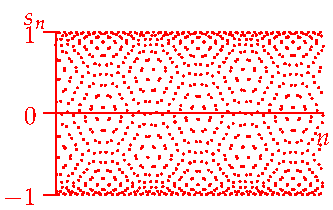
\includegraphics[scale=1]{bwsine}
\end{example}

\goodbreak


\boldsubsubsection{Subsequential Limits, Divergence by Oscillation \& Closed Sets}

Recall Definition \ref{defn:diverge}, where we stated that a sequence $(s_n)$ \emph{diverges by oscillation} if it neither converges nor diverges to $\pm\infty$. We can now give a positive statement of this idea.
\begin{align*}
(s_n) \text{ diverges by oscillation}&\overset{\text{Thm \ref{thm:limbigboth}}}{\iff} \liminf s_n\neq \limsup s_n\\
&\overset{\text{Thm \ref{thm:subseqhard}}}{\iff}(s_n) \text{ has subsequences tending to different limits}
\end{align*}

The word \emph{oscillation} comes from the third interpretation: if $s_1\neq s_2$ are limits of two subsequences, then any tail of the sequence $\{s_n:n>N\}$ contains infinitely many terms arbitrarily close to $s_1$ and infinitely many (other) terms arbitrarily close to $s_2$. The original sequence $(s_n)$ therefore \emph{oscillates} between neighborhoods of $s_1$ and $s_2$. Of course there could be many other \emph{subsequential limits}\ldots



%\boldsubsubsection{Subsequential Limits \& Closed Sets}


\begin{defn}{}{}
	We call $s\in\R\cup\{\pm\infty\}$ a \emph{subsequential limit} of a sequence $(s_n)$ if there exists a subsequence $(s_{n_k})$ such that $\lim\limits_{k\to\infty}s_{n_k}=s$.
\end{defn}

\begin{examples}{}{subseqlim}
	\exstart The sequence defined by $s_n=\frac 1n$ has only one subsequential limit, namely zero. Recall Lemma \ref{lemm:subseqconv}: $\lim s_n=0$ implies that every subsequence also converges to 0.
\begin{enumerate}\setcounter{enumi}{1}
  \item If $s_n=(-1)^n$, then the subsequential limits are $\pm 1$. %One can prove this similarly to the approach in Example \ref*{ex:divergenceeasy}.\ref{ex:divergenceeasy2}: if $\lim\limits_{k\to \infty}s_{n_k}=s\neq\pm 1$, let $\epsilon=\min\{\nm{s-1},\nm{s+1}\}$ for a contradiction\ldots
  \item The sequence $s_n=n^2(1+(-1)^n)$ has subsequential limits 0 and $\infty$.
  \item All positive even integers are subsequential limits of $(s_n)=(2,4,2,4,6,2,4,6,8,2,4,6,8,10,\ldots)$.

%   \item The $A=\{\frac 1n:n\in\N\}$ is not closed since it contains the sequence $s_n=\frac 1n$ whose limit $0$ does not lie in $A$.
%   \item The set $B=A\cup\{0\}$ is closed. The only possible limits of a sequence lying in $B$ is zero.

	\item\label{ex:subseqlim2} (Hard!)\lstsp Recall the countability of $\Q$ from a previous class: the standard argument enumerates the rationals by constructing a sequence
	\[(r_n)=\Bigl(\frac 01,\underbrace{\frac 11,-\frac 11}_{\nm p+q=2}, \underbrace{\frac 12,-\frac 12,\frac 21,-\frac 21}_{\nm p+q=3}, \underbrace{\frac 13,-\frac 13,\frac 31,-\frac 31}_{\nm p+q=4}, \underbrace{\frac 14,-\frac 14,\frac 23,-\frac 23,\frac 32,-\frac 32,\frac 41,-\frac 41}_{\nm p+q=5},\ldots\Bigr)\]
	We claim that the set of subsequential limits of $(r_n)$ is in fact the full set of $\R\cup\{\pm\infty\}$!\smallbreak
	To see this, let $a\in\R$ be given and choose a subsequence $(r_{n_k})$ inductively:
	\begin{itemize}
	  \item By the density of $\Q$ in $\R$ (Corollary \ref{cor:qdense}), the set $S_n=\Q\cap (a-\frac 1n,a+\frac 1n)$ contains infinitely many rational numbers and thus infinitely many terms of the sequence $(r_n)$.
	  \item Choose any $r_{n_1}\in S_1$ and, for each $k\ge 2$, choose any\footnotemark{}
	  \[r_{n_k}\in S_k\text{ \ such that \ }n_k>n_{k-1}\]
	  \item Since $\nm{r_{n_k}-a}<\frac 1k$, we conclude that $\lim\limits_{k\to\infty}r_{n_k}=a$.
% 	  \item By the density of $\Q$ in $\R$ (Corollary \ref{cor:qdense}), the set $S_n=\Q\cap (a-\frac 1n,a+\frac 1n)$ contains infinitely many rational numbers.
% 	  \item Define $n_1=\min\{n:r_n\in S_1\}$ and, for each $k\ge 2$,
% 	  \[n_k:=\min\{n\in\N:n>n_{k-1}\text{ and }\nm{r_n-a}<\tfrac 1k\}\]
% 	  \item For each $k$, $\nm{r_{n_k}-a}<\frac 1k$, from which $\lim\limits_{k\to\infty}r_{n_k}=a$.
	\end{itemize}
	An argument for the subsequential limits $\pm\infty$ is in the Exercises. Somewhat amazingly, the \emph{specific} sequence $(r_n)$ is irrelevant: the conclusion is the same for \emph{any} sequence enumerating $\Q$!
	
	\item (Even harder---Example \ref{ex:sinn}, cont.)\lstsp We won't prove it, but the set of subsequential limits of $(s_n)=(\sin n)$ is the \emph{entire interval} $[-1,1]$! Otherwise said, for any $s\in[-1,1]$ there exists a subsequence $(\sin n_k)$ such that $\lim\limits_{k\to\infty}\sin n_k=s$.
	
% 
% Let $S=\R^+\cap\{a+2\pi b:a,b\in\Z\}$. By Diophantine approximation, there exists a sequence in $S$ such that
% 	\[\frac{a_n}{b_n}\to -2\pi,\qquad a_n+2\pi b_n<\frac 1{b_n} \to 0\]
% 
%  	Let $x\in\R^+\setminus S$ and let $t_1=a_1+2\pi b_1\in S$ satisfy $t_1<\min\{1,x\}$: such exists by convergence. Multiply by $m_1\in\N$ to obtain $m_1t_1<x<(m_1+1)t_1$, let $s_1:=t_1m_1$ and observe that $0<x-s_1\le t_1<1$.\par
% 		Repeat: let $t_2=a_2+2\pi b_2\in S$ satisfy $t_2<\min\{\frac 12,x-t_1m_1\}$. Again multiply by an integer such that $m_2t_2<x-t_1m_1<(m_2+1)t_2$, let $s_2:=s_1+m_2t_2$ and observe that $0<x-s_2<t_2<\frac 12$.\par
% 		Repeat ad infinitum: the process never ceases since $x\not\in S$. We obtain a sequence $(s_n)\subseteq S$ with $n\th$ term $s_n=\sum_{k=1}^nt_km_k$ and where $0<x-s_n<\frac 1n$. We conclude that $(s_n)$ has limit $x$.\smallbreak
% 		Now let $s\in [-1,1]$, define $x=\sin^{-1}s$ and write $s_n=p_n+2\pi q_n$. By the continuity of sine, we see that
% 		\[\sin p_n=\sin s_n\xrightarrow[n\to\infty]{} \sin x=s\]
\end{enumerate}
\end{examples}

\footnotetext{As in the proof of Theorem \ref{thm:subseqhard}, we could make this more explicit by choosing minimums, but there is no need: if there are infinitely many $r_n$ in $S_k$, then only finitely many of them can come before $r_{n_{k-1}}$.}

\goodbreak


\begin{thm}{}{ssqlimit}
Let $(s_n)$ be a sequence in $\R$ and let $S$ be its set of subsequential limits. Then
\begin{enumerate}
  \item $S$ is non-empty (as a subset of $\R\cup\{\pm\infty\}$).
  \item $\sup S=\limsup s_n$ and $\inf S=\liminf s_n$.
  \item $\lim s_n$ exists iff $S$ has only one element: namely $\lim s_n$.
\end{enumerate}
\end{thm}

\begin{proof}
\begin{enumerate}
  \item By Theorem \ref{thm:subseqhard}, $\limsup s_n\in S$.
  \item By part 1, $\limsup s_n\le \sup S$. For any convergent subsequence $(s_{n_k})$, we have $n_k\ge k$, whence
	\[\forall N,\ \{s_{n_k}:k>N\}\subseteq\{s_n:n>N\}\implies \lim s_{n_k}=\limsup s_{n_k}\le\limsup s_n\]
	Since this holds for \emph{every} convergent subsequence, we have $\sup S\le\limsup s_n$, and therefore equality. The result for $\inf S$ is similar.
  \item Applying Theorem \ref{thm:limbigboth}, we see that $\lim s_n$ exists if and only if
  \begin{align*}
		\limsup s_n=\liminf s_n&\iff \sup S=\inf S \iff S\text{ has only one element}\tag*{\qedhere}
	\end{align*}
\end{enumerate}
\end{proof}

\boldinline{Closed Sets}

You should be comfortable with the notion of a \emph{closed interval} (e.g.{} $[0,1]$) from elementary calculus. Using sequences, we can make a formal definition. 

\begin{defn}{}{closed}
	Let $A\subseteq\R$.
	\begin{itemize}
	  \item We say that $s\in\R$ is a \emph{limit point} of $A$ if there exists a sequence $(s_n)\subseteq A$ converging to $s$.
	  \item The \emph{closure} $\cl A$ is the set of limit points of $A$.
	  \item $A$ is \emph{closed} if it equals its closure: $A=\cl A$.
	\end{itemize}
\end{defn}

\begin{examples}{}{}
	\exstart The interval $[0,1]$ is closed. If $(s_n)\subseteq [0,1]$ has $\lim s_n=s$, then
  \[0\le s_n\le 1 \smash[t]{\overset{\text{Thm \ref{thm:limitgreatk}}}{\implies}} s\in [0,1]\]
  More generally, every `closed interval' $[a,b]$ is closed, as are \emph{finite} unions of closed intervals, for instance $[1,5]\cup[7,11]$.
	\begin{enumerate}\setcounter{enumi}{1}
  	\item The interval $(0,1]$ is not closed since its closure is $\cl{(0,1]}=[0,1]$. In particular, the sequence $s_n=\frac 1n$ lies in the original interval but has limit $0$. Indeed this example shows that an \emph{infinite} union of closed intervals need not be closed.
	\end{enumerate}
\end{examples}


\begin{thm}{}{subseqlimitclosed}
If $(s_n)$ is a sequence, then its set of (finite) subsequential limits is closed.
\end{thm}

We omit the proof since it is hard to read, involving unpleasantly many subscripts (subsequences of subsequences\ldots). %The theorem essentially says that one can make a set closed by throwing in all its sequential limits.


\goodbreak


\begin{exercises}{}{}
	\emph{Key concepts/results:\quad ????}
	
	\begin{enumerate}
	  \item%[2.]
	  Consider the sequences with the following $n\th$ terms:
		\[
			a_n=(-1)^n\qquad b_n=\frac 1n\qquad c_n=n^2\qquad d_n=\frac{6n+4}{7n-3}
		\]
		\begin{enumerate}
		  \item For each sequence, give an example of a monotone subsequence.
		  \item For each sequence, state its set of subsequential limits.
		  \item For each sequence, state its $\limsup$ and $\liminf$.
		  \item Which of the sequences converge? diverge to $+\infty$? diverge to $-\infty$?
		  \item Which of the sequences are bounded?
	  \end{enumerate}
  
  
  	\item Prove the case of Lemma \ref{lemm:subseqconv} when $\lim s_n=\infty$
  
% 	  \item%[6.]
% 	  Show that every subsequence of a subsequence of a given sequence is itself a subsequence of the given sequence.

		\item\label{exs:liminfsuplim} Suppose that $\lim s_n=s$ (could be $\pm \infty$). Use Theorem \ref{thm:subseqhard} and Lemma \ref{lemm:subseqconv} to prove that $\limsup s_n=s=\liminf s_n$.\par
		(\emph{This completes the proof of Theorem \ref{thm:limbigboth}})
	
  
		\item Suppose that $L=\lim s_n^2$ exists and is finite.
		\begin{enumerate}
		  \item Given an example of such a sequence where $(s_n)$ is \emph{divergent.}
		  \item Prove that $(s_n)$ contains a convergent \emph{subsequence.} What are the possible limits of this subsequence? Why?\par
		(\emph{Hint: use Bolzano--Weierstraß})
		\end{enumerate}
		
		
		\item\label{exs:bolzano} Complete the third proof of Bolzano--Weierstraß (Theorem \ref{thm:bolzano})  by proving that the constructed subsequence $(s_{n_k})$ is Cauchy.
  
  
  	\item%[9.]
  	\begin{enumerate}
  		\item Show that the closed interval $[a,b]$ is a closed set in the sense of Definition \ref{defn:closed}.
  		\item Is there a sequence $(s_n)$ such that $(0,1)$ is its set of subsequential limits?
  	\end{enumerate}
  
  
  	\item%[7.]
  	Let $(r_n)$ be any sequence enumerating of the set $\Q$ of rational numbers. Show that there exists a subsequence $(r_{n_k})$ such that $\lim\limits_{k\to\infty}r_{n_k}=+\infty$.\par
  	(\emph{Hint: modify the argument in Example \ref*{ex:subseqlim}.\ref{ex:subseqlim2}})
  
  
  	\begin{minipage}[t]{0.55\linewidth}\vspace{0pt}
  	\item%[10.]
  	(Hard)\lstsp Let $(s_n)$ be the sequence of numbers defined in the figure, listed in the indicated order.
  	\begin{enumerate}
		  \item Find the set $S$ of subsequential limits of $(s_n)$.
		  \item Determine $\limsup s_n$ and $\liminf s_n$.
	  \end{enumerate}
  	\end{minipage}\begin{minipage}[t]{0.44\linewidth}\vspace{0pt}
  		\hfill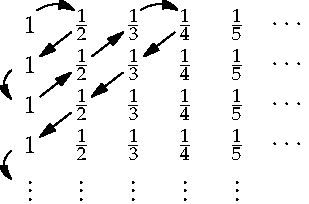
\includegraphics{diag-arg}
  	\end{minipage}
  
  
%   	\item\label{exs:closure} The \emph{closure} $\cl A$ of a set of real numbers $A\subseteq\R$ is the set of limits of all convergent sequences in $A$. Prove that $\cl{(0,1)}=[0,1]$.


	\end{enumerate}
\end{exercises}

\clearpage


\subsection{Lim sup and Lim inf}

In this section we collect a couple of useful results, mostly for later use. First, we observe that the limit laws do not work as tightly for limits superior and inferior.

\begin{thm}{}{}
	Let $(s_n),(t_n)$ be bounded sequences.
	\begin{enumerate}
	  \item $\limsup(s_n+t_n)\le\limsup s_n+\limsup t_n$
	  \item If, in addition, $(s_n)$ is convergent to $s$, then we have equality
	\[\limsup(s_n+t_n)=s+\limsup t_n\]
	\end{enumerate}
\end{thm}

Modifications can be made infima and products of sequences (Exercise \ref{exs:limsupprod}).

\begin{example}{}{}
	To see that equality is unlikely, take $s_n=(-1)^n=-t_n$, then
	\[\limsup(s_n+t_n)=0<2=\limsup s_n+\limsup t_n\]
\end{example}

\begin{proof}
\begin{enumerate}
  \item For each $N$, the set $\{s_n+t_n:n>N\}$ is bounded above by
	\[\sup\{s_n:n>N\}+\sup\{t_n:n>N\}\]
	from which
	\[\sup\{s_n+t_n:n>N\}\le\sup\{s_n:n>N\}+\sup\{t_n:n>N\}\]
	Simply take limits as $N\to\infty$ for the first result.\smallbreak
	
% 	
% 	Now let $(t_{n_k})$ be a subsequence converging to $\limsup t_n$ (exists by Theorem \ref{thm:subseqhard}). Then
% 	\[\lim_{k\to\infty}\bigl(s_{n_k}+t_{n_k}\bigr) =s+\limsup t_n\]
% 	By Theorem \ref{thm:ssqlimit}, $\limsup(s_n+t_n)$ is the supremum of the set of subsequential limits of	$(s_n+t_n)$, whence
% 	\[s+\limsup t_n\le \limsup(s_n+t_n)\]
% 	Combining with ($\ast$) gives the result.
	
	\item By part 1, we already know that
	\[\limsup(s_n+t_n)\le s+\limsup t_n\]
	For the other direction, let $a_n=s_n+t_n$ and apply part 1 again:
	\begin{align*}
	\limsup t_n&=\limsup \bigl((s_n+t_n)-s_n\bigr)\le \limsup (s_n+t_n)+\limsup(-s_n)\\
	&=\limsup(s_n+t_n)-s\tag*{\qedhere}
	\end{align*}
\end{enumerate}
\end{proof}


The next result will be critical when we study infinite series, particularly the ratio and root tests.

\begin{thm}{}{rootratio}
	Let $(s_n)$ be a non-zero sequence. Then
	\[\liminf\nm{\frac{s_{n+1}}{s_n}}\le\liminf\nm{s_n}^{1/n}\le\limsup\nm{s_n}^{1/n}\le \limsup\nm{\frac{s_{n+1}}{s_n}}\]
	In particular, $\displaystyle\lim\nm{\frac{s_{n+1}}{s_n}}=L\implies \lim\nm{s_n}^{1/n}=L$ \hfill$(\dag)$
\end{thm}


\begin{examples}{}{}
	\exstart Here is a quick proof that $\lim n^{1/n}=1$ (recall Theorem \ref{thm:limlaw2}): let $s_n=n$, then
  \[\lim\nm{\frac{s_{n+1}}{s_n}}=\lim\frac{n+1}n=1\implies \lim n^{1/n}=\lim\nm{s_n}^{1/n}=1\]
\begin{enumerate}\setcounter{enumi}{1}
  \item Let $s_n=n!$ and apply the corollary to see that
  \[\lim(n!)^{1/n}=\lim\nm{\frac{s_{n+1}}{s_n}}=\lim(n+1)=\infty\]
\end{enumerate}


\begin{proof}
% 	Choose any $a$ for which $0<a<\liminf\nm{\frac{s_{n+1}}{s_n}}$ (the first inequality is trivial if the left side is zero). Then
% 	\[
% 		\lim_{N\to\infty}\inf\left\{\nm{\frac{s_{n+1}}{s_n}}:n>N\right\}>a\implies\exists 
% 		N\text{ such that }\inf\left\{\nm{\frac{s_{n+1}}{s_n}}:n>N\right\}>a
% 	\]
% 	For any $n>N$, we therefore have
% 	\begin{align*}
% 		\nm{\frac{s_{n+1}}{s_n}}>a&\implies \nm{s_n}\ge a^{n-N-1}\nm{s_{N+1}} \implies \nm{s_n}^{1/n}\ge a\left(a^{-N-1}\nm{s_{N+1}}\right)^{1/n}\\
% 		&\implies \liminf\nm{s_n}^{1/n}\ge a\lim\left(a^{-N-1}\nm{s_{N+1}}\right)^{1/n}=a \tag{$\lim b^{1/n}=1$}
% 	\end{align*}
% 	Since $\liminf\nm{s_n}^{1/n}\ge a$ for all $a<\liminf\nm{\frac{s_{n+1}}{s_n}}$, we conclude the first inequality.\smallbreak
% 	The second inequality is trivial, and the third is similar to the first.
% 	
	Assume $\limsup\nm{\frac{s_{n+1}}{s_n}}=L\neq \infty$ (otherwise the third inequality is trivial) and let $\epsilon>0$. Then
	\[
		\lim_{N\to\infty}\sup\left\{\nm{\frac{s_{n+1}}{s_n}}:n>N\right\}<L+\epsilon\implies\exists 
		N\text{ such that }\sup\left\{\nm{\frac{s_{n+1}}{s_n}}:n>N\right\}<L+\epsilon
	\]
	For brevity, denote $a=L+\epsilon$ and $b=a^{-N-1}\nm{s_{N+1}}$. For any $n>N$, we therefore have
	\begin{align*}
		\nm{\frac{s_{n+1}}{s_n}}<a&\implies \nm{s_n}< a^{n-N-1}\nm{s_{N+1}} \implies \nm{s_n}^{1/n}< a\left(a^{-N-1}\nm{s_{N+1}}\right)^{1/n} =ab^{1/n}\\
		&\implies \limsup\nm{s_n}^{1/n}\le a\lim b^{1/n}=a=L+\epsilon
	\end{align*}
	Since this holds for all $\epsilon>0$, we conclude the third  inequality: $\limsup\nm{s_n}^{1/n}\le L$.\smallbreak
	The second inequality is trivial and the first is similar to the third.
\end{proof}
\end{examples}

\begin{exercises}{}{}
	\emph{Key concepts/results:\quad ????}
	
	%\exstart Compute $\lim \frac 1n(n!)^{1/n}$\vspace{-5pt}
%  and consider $s_n=\frac{n!}{n^n}$. Since
% \[\frac{s_{n+1}}{s_n}=\left(\frac n{n+1}\right)^n=\left(\frac{n+1}n\right)^{-n} = \left(1+\frac 1n\right)^{-n}\to e^{-1}\]
% we conclude that
% \[\lim\nm{s_n}^{1/n}=\lim\frac 1n(n!)^{1/n}=e^{-1}\]
	\begin{enumerate}
  	\item Compute $\lim \frac 1n(n!)^{1/n}$\par
		(\emph{Hint: let $s_n=\frac{n!}{n^n}$ in Theorem \ref{thm:rootratio} and recall that $\lim\left(1+\frac 1n\right)^n=e$})
  
  	\item Evaluate $\lim\left(\frac{(2n)!}{(n!)^2}\right)^{1/n}$
%    Taking $s_n=\dfrac{(2n)!}{(n!)^2}$, we obtain
%   \[\lim\nm{s_n}^{1/n}=\lim\nm{\frac{s_{n+1}}{s_n}} =\lim\frac{(2n+2)!(n!)^2}{(2n)!(n+1)!^2} =\frac{(2n+2)(2n+1)}{(n+1)^2}=4\]
  
  	\item\label{exs:limsupprod} Let $(s_n)$ and $(t_n)$ be non-negative, bounded sequences.
		\begin{enumerate}
			\item Prove that $\limsup(s_nt_n)\le\left(\limsup s_n\right)\left(\limsup t_n\right)$
			\item Give an example which shows that we do not expect equality in part (a).
			\item If, in addition, $\lim s_n=s$, prove that $\limsup(s_nt_n)=s\limsup t_n$.
		\end{enumerate}
% 	
% 	The arguments for these are almost identical to those for sums.
% 	\begin{enumerate}
% 	  \item For each $N$, the set $\{s_nt_n:n>N\}$ is bounded above by
% 		\[\sup\{s_n:n>N\}\sup\{t_n:n>N\}\]
% 		from which
% 		\[\sup\{s_nt_n:n>N\}\le\sup\{s_n:n>N\}\sup\{t_n:n>N\}\]
% 		Now take limits as $N\to\infty$ where we use the limit laws for the right hand side.
% 		\item Let $s_n=1+(-1)^n$ and $t_n=1-(-1)^n$, then $s_nt_n=0$, whence
% 		\[\limsup (s_nt_n)=0<4=(\limsup s_n)(\limsup t_n)\]
% 		\item	Let $(t_{n_k})$ be a subsequence converging to $\limsup t_n$. Then
% 		\[\lim_{k\to\infty}\bigl(s_{n_k}t_{n_k}\bigr) =s\limsup t_n\]
% 		Since $\limsup(s_nt_n)$ is the supremum of the set of subsequential limits of$(s_nt_n)$, we see that
% 		\[s\limsup t_n\le \limsup(s_nt_n)\]
% 		Combining with part (a) gives the result.
% 	\end{enumerate}

		%\item Give an alternative proof 

		\item Consider the sequence with $s_{2m}=s_{2m+1}=2^{-m}$:
		\[(s_n)_{n=0}^\infty=\left(1,1,\frac 12,\frac 12,\frac 14,\frac 14,\frac 18,\frac 18,\ldots\right)\]
		Compute $\nm{s_n}^{1/n}$ and $\nm{\frac{s_{n+1}}{s_n}}$ when $n$ is even and then when it is odd. Thus find all expressions in Theorem \ref{thm:rootratio} and hence conclude that the converse of $(\dag)$ is \emph{false.}


	\end{enumerate}
\end{exercises}

\fi